\begin{refsection}
\hypertarget{verb}{%
\chapter{Verb and verb phrase}\label{chap-verb}}

\section{Introduction}

A number of general concepts are important for a discussion of verbs and verb phrases. Here are some notional definitions (i.e., those based on meaning) for key concepts:
 
\begin{description}[font=\normalfont\scshape]
    \item[verb:] shows the action, existence, or state.\footnote{In linguistics, there is a difference between \emph{verb} and \emph{predicate}, the former referring to the part of speech, while the latter to the part of a sentence. In linguistics problems, however, the term \emph{predicate} is typically not used, and it is usually replaced by \emph{verb}.}
    \item[subject:] typically shows who or what performs the action.
    \item[(direct) object:] typically shows the person or object which is acted upon by the subject.
    \item[indirect object:] shows the entity upon which the action is reflected indirectly.
\end{description}

\noindent We can also think about connections between verbs and noun phrases. For example:

\begin{description}[font=\normalfont\scshape]
    \item[transitive {\normalfont and} intransitive verb:] a transitive verb is one which has a direct object (\cmubdata{I broke the glass}) while an intransitive verb is one which has no direct object (\cmubdata{The baby yawned}). Note that in English we cannot say *\cmubdata{I broke} or *\cmubdata{The baby yawned his mouth}. Some verbs can vary in whether they take a direct object: thus, the verb \cmubdata{to eat} can be both transitive (\cmubdata{She is eating a pizza} -- transitive use of \cmubdata{eat}, with \cmubdata{a pizza} as the direct object) and intransitive (\cmubdata{She is eating}).
\end{description}

\section{Variables of the verb}\largerpage[2]

By variables, we mean those parameters which change in the problem. For example, comparing the sentences:

\exrule{\cmubdata{He eats.} \hspace{7em} \cmubdata{I ate.}}

\noindent we notice that the variables are \textit{subject} (\cmubdata{he} vs. \cmubdata{I}), tense (present vs. past), but not the verb itself (both sentences have the same verb - \cmubdata{eat}).

Generally, these variables can be classified into three categories:

\begin{enumerate}
    \item TAM (Tense, Aspect, Mood)
    \item Arguments (S, S+O, S+O+O) 
    \item Others
\end{enumerate}

\section{TAM (Tense, Aspect, Mood)} 
\subsection{Tense} 
Tense is a grammatical category, related to the concept of time. Languages often have three subtypes of tense: past (often used when the action or state denoted by the verb occurs before the moment of speech), present (action happens while speaking) and future (action will take place after the moment of speech).

Although most of the Indo-European languages have all of these tenses, there are languages which only have two distinct tenses. Thus, there are languages which only distinguish \textit{past} and \textit{non-past}, such as Arabic and Japanese (non-past refers to everything that is not past, thus representing present and future) or languages which distinguish \textit{future} and \textit{non-future}, such as Greenlandic or Nivkh (where non-future represents past and present), or even languages that distinguish only \textit{present} and \textit{non-present} (one example is the constructed language Ithkuil). Moreover, there can be languages which make no tense distinctions at all, such as Chinese or Dyirbal.

Although there are only three broad categories of tense, some languages can have many more actual tenses, mainly depending on the specific moment at which the action occurred. For example, the Yagua language has five different past tense markers:\footnote{This phenomenon was featured in a problem by Vlad A. Neacșu (RoLO 2018).}

\begin{enumerate}[label = \alph*.]
    \item \cmubdata{-jásiy} -- for actions which took place a couple of hours ago (in the same day);
    \item \cmubdata{-jay} -- for actions occurring one day ago;
    \item \cmubdata{siy} -- one week to one month ago;
    \item \cmubdata{tíy} -- one or two months to one or two years ago; 
    \item \cmubdata{-jada} -- more than two years ago (it is also called \textit{distant past} or \textit{legendary past}).  
\end{enumerate}

 Additionally, some languages can have specific tenses, e.g., specific for actions occurring one day ago, the previous day (\textit{hesternal} tense) or the following day (\textit{crastinal} tense). There can even be \textit{pre-hesternal} and \textit{post-crastinal} tenses, referring to actions occurring two days before/after the moment of speech.

Some languages also have \textit{hodiernal} tenses, which are specific to actions occurring on the same day as the moment of speech (today). These can be past tenses (actions happening earlier today) or future tenses (actions happening later today).

Therefore, returning to the Yagua example, we can define the marker a. (\cmubdata{-jásiy}) as a past hodiernal tense, while b. (\cmubdata{-jay}) can be considered a hesternal tense marker.

\subsection{Aspect}

 Aspect shows the evolution in time of an action, state or event, independent of the moment of speech. The most common aspects are the \textit{perfective} and \textit{imperfective}.

Perfective aspect is used when the event denoted by the verb is bounded. The imperfective is used when the event is seen as unfolding, or when the event is repeated/habitual. Depending on the language, there can also be other aspects such as:
\begin{itemize}
    \item \textsc{Progressive} = action is unfolding (progressing).
    \item \textsc{Semelfactive} = action is short-term.
    \item \textsc{Accidental} = action is done by mistake.
\end{itemize}

 There are a lot of different aspects and their meaning can usually be inferred from their name (\textit{punctual}, \textit{resumptive}, \textit{intensive}, \textit{attenuative}, \textit{moderative}, \textit{experiential}, \textit{durative}, \textit{pausative}, \textit{terminative}, \textit{episodic}, \textit{generic}, \textit{habitual}, \textit{discontinuous}, \textit{prospective}, \textit{intentional}, etc.). Memorising the names of all these aspects is not necessary, but it is important that you get used to the different meanings these aspects convey. Moreover, all of these aspects (not all of which exist in English so they may be expressed in more roundabout ways) need to be translated into English in a linguistics problem (most likely through a specific phrasing or by using an adverb). Therefore, instead of referring to the aspect itself, when solving a linguistics problem, you can simply write “The structures which are translated as...”. For example, the durative aspect can be translated into English by phrases such as \texttr{for a while}. Therefore, even if you do not know the name of the aspect (\textit{durative}), it is enough to realise that there is a distinction between, for example, \cmubdata{You ate} and \cmubdata{You ate for a while}, in which case you can explain the sense of the durative aspect marker through the phrase \cmubdata{for a while}. Other examples are: potential aspect \cmubdata{probably}, prospective aspect \cmubdata{I'm getting ready to...}, etc.

\remember{In English, at least at school, aspect is not often talked about and the idea of “tense”\ refers, in fact, to a combination of tense and aspect. English has two main aspects: perfect aspect (e.g., \cmubdata{I have/had eaten a sandwich}, as defined above) and progressive aspect (e.g., \cmubdata{I am/was eating a sandwich}, sometimes known as continuous aspect).
}

\subsection{Mood}

 Mood is an inflectional category related to the concept of modality, which is often connected with the speaker's attitude towards the message being transmitted (whether it is a fact, a wish, a command, etc.). Moods are classified into two broad classes: \textit{realis} moods which show that something is a statement or a fact; and \textit{irrealis} moods which refer to actions which have not happened (or will certainly not happen).

\subsubsection{Realis moods}

\begin{enumerate}
    \item Indicative mood: It is the most common mood and it is used for statements of fact. It is considered that all situations in a particular language that cannot be categorised as another mood will be classified as belonging to the indicative mood. 
    \item Certain languages can have another realis mood, a special mood which is used solely for general truths, as in the examples \cmubdata{Fish swim} or \cmubdata{Chickens have two legs.} 
\end{enumerate}

\subsubsection{Irrealis mood}

There are many different subtypes of irrealis. As with the Uralic cases listed in \sectref{sec:variables-of-the-noun}, there is no need for you to remember all these subtypes. However, some subtypes appear more frequently in linguistics problems and we briefly describe these below.
\begin{enumerate}
    \item Subjunctive mood: marks imaginary/hypothetical events, as well as opinions and emotions. It is the main irrealis mood and it represents an “um\-brel\-la term”\ for all the instances in which one language does not have another mood to express that attitude. 
    \item Conditional mood: the action is conditioned (by another action). 
    \item Optative mood: shows desires or wishes.
    \item Imperative mood: direct commands/request/interdictions.
    \item Jussive mood: similar to the imperative, but it expresses commands towards a third person, not present. Since in English this mood is not expressed directly by the verb, we usually use the subjunctive mood to express a similar meaning, e.g., \cmubdata{I asked that he cook.}
\end{enumerate}

\subsection{Verbal expression of modality}

 In certain languages, modal verbs are used to express different kinds of modality. In many languages, modal verbs are considered auxiliary verbs. This means that they are accompanied by a ``lexical verb'', i.e., a verb with semantic content. In English, the central modal verbs (such as \cmubdata{must} and \cmubdata{should}) take the plain form of the verb as their complement (e.g., \cmubdata{I must leave}, \cmubdata{you should eat}). They can also combine with aspect markers (\cmubdata{he must be working}, \cmubdata{she should have stayed}): notice here that it is the following verb (the aspect marker) that is unchanged; the form of the lexical verb is determined by the aspect marker (\cmubdata{be $+ V$ing}, \cmubdata{have $+ V$ed}).

 Other verbs can also be used to express modality, and such verbs often take the \cmubdata{to}-infinitive as their complement. For example, in the sentence \cmubdata{I want to go}, \cmubdata{want} is the verb which shows the modality (the desire), while \cmubdata{go} is the verb with semantic content, showing the action I \textit{want/desire} to perform. Other such patterns in English include \cmubdata{wish to $V$}, \cmubdata{try to $V$}, etc.

The verbs in bold in sentences like \cmubdata{I \textbf{want} to swim} and \cmubdata{I \textbf{tried} to swim} are sometimes known as catenative verbs because they can form a sequence or chain of verbs (\textit{catena} is Latin for \texttr{chain}), as in \cmubdata{I \textbf{want} to \textbf{try} to swim}. Catenative verbs take a non-finite verb (e.g., an infinitive or participle) as their complement in English. Such catenative verbs can express modality (\cmubdata{I \textbf{need} to leave}) and aspect (\cmubdata{He \textbf{kept} swimming}), and since catenative verbs can combine, a sentence can involve the marking of both modality and aspect (\cmubdata{I \textbf{need} to \textbf{keep} swimming}).

This concept is relevant because it involves an interdependency between the two verbs, which are grammatically and semantically interconnected. Thus, in linguistics problems, if sequences of verbs occur, we need to pay attention to the following potential parameters: the order of the modal/catenative verb and the semantic verb (whether it comes before or after it, or whether there are other words or morphemes in between), as well as which of the two verbs gets conjugated (in some languages, only the auxiliary verbs are conjugated; in others, only the lexical verb; and in yet others, both the auxiliary and the lexical verb are conjugated).

\subsection{Evidentiality}

 Evidentiality, unlike tense, aspect, and mood, shows the way in which the uttered information was discovered or, in other words, what evidence there is for the transmitted information. For example, in Pomo, there are four types of evidentiality, each of them having its own marker:

\begin{enumerate}
    \item Visual: the speaker witnessed the action;
    \item Sensorial non-visual: the speaker felt (by hearing, smelling, etc.) something that pointed towards the action. For example, the sentence \cmubdata{The kids fought} can receive a sensorial non-visual evidentiality marker to point out that the speaker has not seen the children fighting, but heard them;
    \item Inferential: the speaker did not witness the action but was able to see its consequence or result. For example, the sentence \cmubdata{The man cooked the fish} can carry an inferential evidentiality marker to show that the speaker has not seen the fish being cooked (the process of cooking), but, for example, saw someone holding a plate with the cooked fish (thus, being able to infer that, at some point, the fish went through the cooking process).
    \item Reportative: the speaker found out the information from someone else. 
\end{enumerate}

 For example, the English sentence \cmubdata{It rained} could be translated into Pomo in four different ways, depending on the source of the evidence. Visual -- the speaker sees that it's raining; sensorial non-visual -- they hear the rain; inferential -- they notice it is wet outside; reportative -- someone tells them it rained.

Other evidential contrasts can be:

\begin{enumerate}[resume]\sloppy
    \item Witness vs. non-witness: the speaker witnessed the action (the information was retrieved through direct observation) or not. This type of evidentiality occurs in Turkish, where there are two types of past, called \textit{seen past} (\cmubdata{görülen geçmiş zaman}, witness evidentiality marker) and \textit{heard past} (\cmubdata{duyulan geçmiş zaman}, non-witness evidential).
    \item First-hand vs. second-hand vs. third-hand: first-hand information is equivalent to directly observed information (witness); second-hand information is used to show that the speaker found out the information from someone else (who witnessed the action), while third-hand information indicates that the speaker found out the information from another person (who, in turn, found it out from a third person who witnessed the action).
\end{enumerate}

 As in the case of TAM categories, there can be other evidential markers and, depending on the language, each of these categories can be further divided into subcategories. For example, the inferential evidential can have the following subtypes: information deduced based on direct evidence (seeing the result of the action), information deduced based on general knowledge, information deduced (or inferred) based on the speaker's past experiences in similar situations, etc.

Moreover, evidentiality can also be combined with tense, aspect, and mood, for which reason some linguists prefer using the abbreviation TAME (instead of TAM): tense, aspect, mood, evidentiality.

\section{Arguments}

 In many linguistics problems, we need to identify the arguments of the verb. These are often the subject (S) and object(s) (O) of the verb. In some cases, we also distinguish between the subject of an intransitive verb and that of a transitive verb. This will be discussed more thoroughly in \sectref{morphoalign}.

 In verb (phrase) problems, S and O are often expressed as pronouns in the English translations, though they may be directly attached to the verb as affixes in the target language. Depending on the difficulty of the problem, we can have different situations:

\begin{itemize}
    \item Easy problems: subject and object are marked through distinct, independent affixes.
    \item Medium problems: in which S and O are either combined into a single affix, or they undergo certain phonological changes.
    \item Hard problems: in which S and O are not expressed uniquely, but rather through a combination of affixes. 
\end{itemize}
For more information about case alignment, see \sectref{morphoalign}.

\begin{problem}{\langnameSwahili}{\nameRSim}{\PrincetonAbbr}
\IntroVerbs{\langnameSwahili}\ \IntroAndEnglish:
\begin{center}
\begin{tabular}{rll}
     \sentlineonerow{Ninasema.}{I speak.}
     \sentlineonerow{Wunasema.}{You speak.}
     \sentlineonerow{Anasema.}{She speaks.}
     \sentlineonerow{Wanasema.}{They speak.}
     \sentlineonerow{Ninaona.}{I see.}
     \sentlineonerow{Niliona.}{I saw.}
     \sentlineonerow{Ninawaona.}{I see them.}
     \sentlineonerow{Niliwuona.}{I saw you.}
     \sentlineonerow{Ananiona.}{She sees me.}
     \sentlineonerow{Wutakaniona.}{You will see me.}
     \sentlineonerow{\pbblank}{She saw them.}
     \sentlineonerow{\pbblank}{I will see you.}
     \sentlineonerow{\pbblank}{She saw me.}
\end{tabular}
\end{center}
\begin{assgts}
\item \fillblanks
\end{assgts}
\end{problem}

\begin{mysolution}
 We notice that all English examples containing the verb \texttr{to see} end in \cmubdata{ona} in Swahili. Similarly, all English examples which contain the subject \texttr{I} start with \cmubdata{ni} in Swahili. Separating these two morphemes, we obtain:

\begin{center}
\begin{longtable}{rll}
\setcounter{exx}{0}
     \sentlineonerow{Ni-nasema.}{I speak.}
     \sentlineonerow{Wunasema.}{You speak.}
     \sentlineonerow{Anasema.}{She speaks.}
     \sentlineonerow{Wanasema.}{They speak.}
     \sentlineonerow{Ni-na-ona.}{I see.}
     \sentlineonerow{Ni-li-ona.}{I saw.}
     \sentlineonerow{Ni-nawa-ona.}{I see them.}
     \sentlineonerow{Ni-liwu-ona.}{I saw you.}
     \sentlineonerow{Anani-ona.}{She sees me.}
     \sentlineonerow{Wutakani-ona.}{You will see me.}
\end{longtable}
\end{center}

In examples 5 and 6 we are left with only one unidentified morpheme (\cmubdata{na} and \cmubdata{li}, respectively). The two sentences differ only in terms of their tense (past vs. present); therefore, we infer that \cmubdata{na} is the present-tense marker, while \cmubdata{li} is the past-tense marker. Separating these two morphemes, we obtain:

\begin{center}
\begin{longtable}{rll}
\setcounter{exx}{0}
     \sentlineonerow{Ni-na-sema.}{I speak.}
     \sentlineonerow{Wu-na-sema.}{You speak.}
     \sentlineonerow{A-na-sema.}{She speaks.}
     \sentlineonerow{Wa-na-sema.}{They speak.}
     \sentlineonerow{Ni-na-ona.}{I see.}
     \sentlineonerow{Ni-li-ona.}{I saw.}
     \sentlineonerow{Ni-na-wa-ona.}{I see them.}
     \sentlineonerow{Ni-li-wu-ona.}{I saw you.}
     \sentlineonerow{A-na-ni-ona.}{She sees me.}
     \sentlineonerow{Wutakani-ona.}{You will see me.}
\end{longtable}
\end{center}

Now it is easy to identify that the morpheme order is Subject – Tense – Object – Stem (we can abbreviate it as S-Tense-O-V). Moreover, we notice that the subject and object markers are identical. Therefore, we can segment example 10 as well (knowing that \texttr{you} is \cmubdata{-wu-}, and \texttr{I/me} is \cmubdata{-ni-}) and we get \cmubdata{Wu-taka-ni-ona}. Therefore, the future marker is \cmubdata{taka}.

Once all the rules are discovered, it is time to structure them neatly. Usually, in this type of problem, we start by writing down the morpheme order, followed by explaining each of the morphemes.

\subsubsection*{Rules: Option 1}
\begin{itemize}
    \item Structure: S--Tense--O--V
    \item S: 1\textsc{sg} = \cmubdata{ni}, 2\textsc{sg} = \cmubdata{wu}, 3\textsc{sg} = \cmubdata{a}, 3\textsc{pl} = \cmubdata{wa}
    \item Tense: present = \cmubdata{na}, past = \cmubdata{li}, future = \cmubdata{taka}
    \item O: 1\textsc{sg} = \cmubdata{ni}, 2\textsc{sg} = \cmubdata{wu}, 3\textsc{sg} = \cmubdata{a}, 3\textsc{pl} = \cmubdata{wa}
    \item Verb: \texttr{speak} = \cmubdata{sema}, \texttr{see} = \cmubdata{ona}
\end{itemize}

 Another option is combining the order of the morphemes with their structure, in a single table.

\subsubsection*{Rules: Option 2}

\begin{table}
    \begin{tabular}{cccc}
    \lsptoprule
    S & Tense & O & V \\
    \midrule
    \begin{tabular}[t]{l@{~=~}l}
        \cmubdata{ni} & 1\textsc{sg} \\ 
        \cmubdata{wu} & 2\textsc{sg} \\ 
        \cmubdata{a}  & 3\textsc{sg} \\ 
        \cmubdata{wa} & 3\textsc{pl}
    \end{tabular} & 
    \begin{tabular}[t]{l@{~=~}l}
         \cmubdata{li}   & past \\ 
         \cmubdata{na}   & present \\ 
         \cmubdata{taka} & future 
     \end{tabular} & 
     \begin{tabular}[t]{l@{~=~}l}
        \cmubdata{ni} & 1\textsc{sg} \\ 
        \cmubdata{wu} & 2\textsc{sg} \\ 
        \cmubdata{a}  & 3\textsc{sg} \\ 
        \cmubdata{wa} & 3\textsc{pl}
    \end{tabular}& 
    \begin{tabular}[t]{l@{~=~}l}
         \cmubdata{sema} & speak \\ 
         \cmubdata{ona} & see
    \end{tabular}\\
    \lspbottomrule
    \end{tabular}
    \end{table}

 The main disadvantage of these two options (in the case of this problem) is that we have to write the pronoun markers twice (once for S and once for O), although they are identical.

Usually, when we work with pronoun markers, it is favourable to structure them in a table in which we write the person in columns and the number in rows (or vice versa). Therefore, the subject markers become:

\begin{center}
    \begin{tabular}{ cccc }
    \lsptoprule
    & 1 & 2 & 3 \\
    \midrule
    \textsc{sg} & \cmubdata{ni} & \cmubdata{wu} &\cmubdata{a}\\
    \textsc{pl} & & & \cmubdata{wa} \\
    \lspbottomrule
    \end{tabular}
\end{center}

 In this way, we can show the fact that the subject is identical to the object.

\subsubsection*{Rules: Option 3}
\begin{itemize}
    \item Structure: S--Tense--O--V
    \item S = O \hspace{5em}  \begin{tabular}{ cccc }
    \lsptoprule
    & 1 & 2 & 3 \\
    \midrule
    \textsc{sg} & \cmubdata{ni} & \cmubdata{wu} &\cmubdata{a}\\
    \textsc{pl} & & & \cmubdata{wa} \\
    \lspbottomrule
    \end{tabular}
    \item Tense: present = \cmubdata{na}, past = \cmubdata{li}, future = \cmubdata{taka}
    \item Verb: \texttr{speak} = \cmubdata{sema}, \texttr{see} = \cmubdata{ona}
\end{itemize}

 All these options for writing out the rules are correct and complete, and they would all receive the maximum score. But, depending on the problem, one of them fits better in the sense that it is more succinct and helps save some time.

Once the rules are written, we can start solving the tasks.

\begin{center}
    \begin{tabular}{rll}
         11. & 3\textsc{sg}--past--3\textsc{pl}--\texttr{see} & \texttr{She saw them.}\\
         12. & 1\textsc{sg}--future--2\textsc{sg}--\texttr{see} & \texttr{I will see you.}\\
         13. & 3\textsc{sg}--past--1\textsc{sg}--\texttr{see} & \texttr{She saw me.}\\
    \end{tabular}
\end{center}

 Thus, the answers are: 11. \cmubdata{aliwaona} \hfill 12. \cmubdata{nitakawuona} \hfill 13. \cmubdata{aliniona}

\section{Segmenting}

 Segmenting is probably the most important part for this type of problem. It refers to dividing the verb into all its component morphemes, as we did in the previous problem (we divided the word \cmubdata{wutakaniona} into \cmubdata{wu-taka-ni-ona}, so we segmented it into its components).

For simple problems, once the verbs are fully (and correctly) segmented, it is just a matter of making the correspondences and figuring out the meaning of each morpheme. Sometimes segmentation can be complicated due to morphemes that undergo phonological changes.

In the case of chaos-and-order problems (those in which the data are given in random order), the general approach includes: 1) segmenting the verb, 2) deducing the verb structure (in the given language), 3) showing a frequency table.

\end{mysolution}
\begin{problem}{\langnameDabida}{\nameKGilyarova}{\LOYear{\TurLomAbbr}{2006}}
\IntroVerbs{\langnameDabida}\ \IntroAndEnglishRandom:

\begin{exe}
\sn[]{\raggedright
    \cmubdata{dichakaδana}, \cmubdata{βichanirasha}, \cmubdata{kuchanikunda}, \cmubdata{dichakurasha}, \cmubdata{dicharashana},
    \cmubdata{βichamukunda}, \cmubdata{muchadikaδa}, \cmubdata{βichakaδana}
    \glt \texttr{we will argue}, \texttr{you\pl\ will beat us}, \texttr{we will curse you\sg}, \texttr{they will fight}, \texttr{they will curse me},
    \texttr{they will fall in love with you\pl}, \texttr{we will fight}, \texttr{you\sg\ will fall in love with me}}
\end{exe}

\begin{assgts}
\item \detcorr
\item \transinen
\begin{enumerate}
    \item \cmubdata{nichakukaδa}
    \item \cmubdata{βichakundana}
\end{enumerate}
\item \transinen[\langnameDabida]
\begin{enumerate}[start = 3]
    \item \texttr{you\pl\ will argue}
    \item \texttr{you\sg\ will curse them}
\end{enumerate}
\end{assgts}
\end{problem}

\begin{mysolution}
  \begin{description}
    \item[Step 1.] Segmenting: when segmenting the verbs, we are not yet too concerned with the English translations. For this problem, we can start with the special characters since they are the easiest to follow. If we start with the letter \cmubdata{β}, we notice that it appears in three examples and in each of these examples we can separate the morpheme \cmubdata{βicha}. Nevertheless, we need to notice that the morpheme \cmubdata{-cha-} appears in every single given example. Therefore, it most likely represents a separate morpheme. Separating the morphemes \cmubdata{-cha-} and \cmubdata{-βi-} we get:

\begin{center}
    \cmubdata{di-cha-kaδana}, \cmubdata{βi-cha-nirasha}, \cmubdata{ku-cha-nikunda}, \cmubdata{di-cha-kurasha}, \cmubdata{di-cha-rashana},
    \cmubdata{βi-cha-mukunda}, \cmubdata{mu-cha-dikaδa}, \cmubdata{βi-cha-kaδana}
\end{center}

 Next, we notice the repeated strings \cmubdata{-rasha-}, \cmubdata{-kunda-}, and \cmubdata{-kaδa-}, obtaining:

\begin{center}
    \cmubdata{di-cha-kaδa-na}, \cmubdata{βi-cha-ni-rasha}, \cmubdata{ku-cha-ni-kunda}, \cmubdata{di-cha-ku-rasha}, \cmubdata{di-cha-rasha-na},
    \cmubdata{βi-cha-mu-kunda}, \cmubdata{mu-cha-di-kaδa}, \cmubdata{βi-cha-kaδa-na}
\end{center}

 \item[Step 2.] Now we can deduce the Dabida verb structure:

\begin{center}
    \begin{tabular}{|c|c|c|c|c|}
    \hline
    \begin{tabular}{c}
    \cmubdata{di} \\\cmubdata{βi} \\\cmubdata{ku} \\\cmubdata{mu} \\
    \end{tabular} & \begin{tabular}{c}
    \cmubdata{cha} \\
    \end{tabular} & \begin{tabular}{c}
    \cmubdata{di} \\\cmubdata{ni} \\\cmubdata{ku} \\\cmubdata{mu} \\ $\varnothing$ \\
    \end{tabular} & \begin{tabular}{c}
    \cmubdata{kaδa} \\\cmubdata{rasha} \\\cmubdata{kunda} \\
    \end{tabular} & \begin{tabular}{c}
    \cmubdata{na} \\ $\varnothing$ \\\end{tabular}\\
    \hline
    \end{tabular}
\end{center}
\end{description}
\remember{In case of morphemes 3 and 5, it is important to also mark $\varnothing$ (the null morpheme), meaning that the morpheme is optional and it does not appear in all examples.}

\begin{description}
 \item[Step 3.]\sloppy Checking the English examples, we notice only three variables: subject (\texttr{you\sg}, \texttr{we}, \texttr{you\pl}, \texttr{they}), object ($\varnothing$, \texttr{me}, \texttr{you\sg}, \texttr{us}, \texttr{you\pl}) and verb (\texttr{to fight}, \texttr{to argue}, \texttr{to beat}, \texttr{to curse}, \texttr{to fall in love}). The tense is not a variable since all examples are in the future tense. We can probably assume that the morpheme \cmubdata{-cha-}, which appears in every single example, is the mark of the future.
\end{description}

\remember{For a correct and complete set of rules, we do not need to write the meaning of that morpheme, since it appears in all examples. Actually, we have no proof that it indicates future tense; we have no evidence as to what its function is as there are no contrasting examples without it.}

 Moreover, we can make some preliminary observations in order to help deduce what is the purpose of each morpheme. We notice that morphemes 1 and 3 are extremely similar (both of them can be \cmubdata{-di-}, \cmubdata{-ku-}, \cmubdata{-mu-}). Therefore, we can guess that these mark the subject and the object (both have the same markers, similar to the previous problem). Moreover, the long morpheme is, usually, the stem (morpheme 4). Nevertheless, we notice that in Dabida we have only three stems, while in English we have five.

We make a frequency table for morphemes 1 and 3 (which we presumed correspond to the pronouns):

\begin{table}[H]
    \hfill
        \begin{tabular}{lcc}
        \lsptoprule
               & \multicolumn{2}{c}{Dabida} \\\cmidrule{2-3}
        Morpheme  & 1\textsuperscript{st} & 3\textsuperscript{rd} \\\midrule
        \cmubdata{di} & 3 & 1 \\
        \cmubdata{βi} & 3 &   \\
        \cmubdata{ku} & 1 & 1 \\
        \cmubdata{mu} & 1 & 1 \\
        \cmubdata{ni} &  & 2  \\
        $\varnothing$ &  & 3  \\
    \lspbottomrule
    \end{tabular}\hfill    
    \begin{tabular}{lcc}
    \lsptoprule
             & \multicolumn{2}{c}{English} \\ \cmidrule{2-3}
     Pronoun& S & O \\\midrule
     1\textsc{sg} &  & 2 \\
     2\textsc{sg} & 1 & 1 \\
     1\textsc{pl} & 3 & 1 \\
     2\textsc{pl} & 1 & 1 \\
     3\textsc{pl} & 3 &  \\
     $\varnothing$ & & 3 \\
     \lspbottomrule
    \end{tabular}\hfill\hbox{}
\end{table}

 In other words, this table shows, for example, that the morpheme \cmubdata{di} in Dabida appears in three examples in the first position and in a single example in the third position. In English, we have only one pronoun which matches this 3-and-1 pattern, namely the second person singular (2\textsc{sg}, \texttr{you\sg}).

We can easily notice that the first morpheme in Dabida corresponds to the subject in English while the third morpheme corresponds to the object. Moreover, we can infer that \cmubdata{-di-} = 1\textsc{pl}, \cmubdata{-ni-} = 1\textsc{sg}, and \cmubdata{-βi-} = 3\textsc{pl}. From the table, we cannot match the 2\textsc{sg} and 2\textsc{pl} since they both appear only once as a subject and once as an object. We can sum up what we have gathered so far as follows:

\exrule{Structure: S-\cmubdata{cha}-O-?-?}
\exrule{S = O: \cmubdata{-di-} = 1\textsc{pl}, \cmubdata{-ni-} = 1\textsc{sg}, and \cmubdata{-βi-} = 3\textsc{pl}, \{\cmubdata{-ku-}, \cmubdata{-mu-}\} = \{2\textsc{sg}, 2\textsc{pl}\}.}

In order to deduce the markers for 2\textsc{sg} and 2\textsc{pl}, we can make a bidimensional frequency table in which we mark the combinations of subject and object:

\begin{table}[H]
  \begin{floatrow}
    \ttabbox{%
    \begin{tabular}{ccccc}
        \lsptoprule
        O / S           & 2\textsc{sg} & \cmubdata{-di-} & 2\textsc{pl} & \cmubdata{-βi-}\\\midrule
        ∅              &     & XX &   & X\\
        \cmubdata{-ni-} & X   &    &   & X\\
        2sg             &     & X  &   &  \\
        \cmubdata{-di-} &     &    & X & X\\
        2pl             &     &    &   &  \\
        \lspbottomrule
    \end{tabular}}{}
    \ttabbox{%
        \begin{tabular}{ccccc}
        \lsptoprule
         O / S & 2sg & 1pl & 2pl & 3pl \\\midrule
        ∅ &  & XX &  & X \\  
       1sg & X &  &  & X \\
       2sg &  & X &  &  \\ 
       1pl &  &  & X & X \\
       2pl &  &  &  &  \\
       \lspbottomrule
         \end{tabular}
    }{}
  \end{floatrow}
\end{table}

For instance, this table shows that we have only one example in which 1\textsc{pl} is subject and 2\textsc{sg} is object, and two examples in which 1\textsc{pl} is subject and there is no object. Since we already know the morphemes for 1\textsc{sg}, 1\textsc{pl} and 3\textsc{pl}, we notice that 2\textsc{sg} is the only person which appears as an object in an example in which 1\textsc{pl} is subject. Therefore we deduce that \cmubdata{-ku-} = 2\textsc{sg} and \cmubdata{-mu-} = 2\textsc{pl}. Based on these results, we can make almost all the correspondences (save for the two examples which both have 1\textsc{pl} as subject and have no object).
\begin{center}
    \begin{tabular}{lcl}
         \cmubdata{βichanirasha} & = & \texttr{They will curse me.} \\
         \cmubdata{kuchanikunda} & = & \texttr{You\sg\ will fall in love with me.} \\
         \cmubdata{dichakurasha} & = & \texttr{We will curse you\sg.} \\
         \cmubdata{βichamukunda} & = & \texttr{They will fall in love with you\pl.} \\
         \cmubdata{muchadikaδa} & = & \texttr{You\pl\ will beat us.} \\
         \cmubdata{βichakaδana} & = & \texttr{They will fight.} \\
    \end{tabular}
\end{center}

\begin{sloppypar}
The two remaining examples are \{\cmubdata{dicharashana}, \cmubdata{dichakaδana}\} = \{\texttr{We will fight.}, \texttr{We will argue.}\}
\end{sloppypar}

It is time to analyse the fourth morpheme (which we previously assumed represents the stem):

\begin{table}[H]
    \begin{tabularx}{\textwidth}{lQl}
    \lsptoprule
    \cmubdata{rasha} & \cmubdata{kunda} & \cmubdata{kaδa} \\
    \midrule
     \texttr{They will curse me.}&\texttr{You\sg\ will fall in love with me.} & \texttr{You\pl\ will beat us.}\\
    \texttr{We will curse you\sg.} &\texttr{They will fall in love with you\pl.} & \texttr{They will fight.}\\
    \lspbottomrule
    \end{tabularx}
\end{table}

 We notice that \wordtrans{-kunda-}{to fall in love}, and \wordtrans{-rasha-}{to curse}. On the other hand, \cmubdata{-kaδa-} seems to mean both \texttr{to fight} and \texttr{to beat}, which, we notice, have similar meanings in English. Since one of the remaining examples contains the verb \texttr{to fight}, it will certainly correspond to the phrase containing \cmubdata{-kaδa-}.

	Therefore, we can make the correspondences:

 \begin{center}
 \begin{tabular}{lcl}
         \cmubdata{βichanirasha} & = & \texttr{They will curse me.} \\
         \cmubdata{kuchanikunda} & = & \texttr{You\sg\ will fall in love with me.} \\
         \cmubdata{dichakurasha} & = & \texttr{We will curse you\sg.} \\
         \cmubdata{βichamukunda} & = & \texttr{They will fall in love with you\pl.} \\
         \cmubdata{muchadikaδa} & = & \texttr{You\pl\ will beat us.} \\
         \cmubdata{βichakaδana} & = & \texttr{They will fight.} \\
         \cmubdata{dicharashana} & = & \texttr{We will argue.} \\
         \cmubdata{dichakaδana} & = & \texttr{We will fight.} \\
    \end{tabular}
\end{center}

 Based on these, we notice that the stem \cmubdata{-rasha-} can have two translations: \texttr{to argue} and \texttr{to curse}. In order to understand when to use one and when to use the other, we carefully analyse the examples containing \cmubdata{-rasha-}. We notice that sentences which do not have a direct object are translated with \texttr{to argue}, while those which have an object use \texttr{to curse}. Similarly, \cmubdata{-kaδa-} means \texttr{to fight} if there is no direct object, or \texttr{to beat} if there is one. Therefore, the meaning of the stem depends on the transitivity of the verb. We can write:

\exrule{\cmubdata{rasha} = \texttr{to argue} (intransitive), \texttr{to curse} (transitive)}
\exrule{\cmubdata{kunda} = \texttr{to fall in love}}
\exrule{\cmubdata{kaδa} = \texttr{to fight} (intransitive), \texttr{to beat} (transitive)}

We come back to the only morpheme left, the fifth one. In order to figure out its function, we make a table in which we separate the structures which contain it from those which do not:

\begin{table}[H]
    \begin{tabular}{l @{~=~} l }
    \lsptoprule
    \multicolumn{2}{c}{\cmubdata{-na}}\\
    \midrule
         \cmubdata{βichakaδana}  & \texttr{They will fight.} \\
         \cmubdata{dicharashana} & \texttr{We will argue.} \\
         \cmubdata{dichakaδana}  & \texttr{We will fight.} \\
    \midrule
    \multicolumn{2}{c}{$\varnothing$}\\
    \midrule
         \cmubdata{βichanirasha} & \texttr{They will curse me.} \\
         \cmubdata{kuchanikunda} & \texttr{You\sg\ will fall in love with me.} \\
         \cmubdata{dichakurasha} & \texttr{We will curse you\sg.} \\
         \cmubdata{βichamukunda} & \texttr{They will fall in love with you\pl.} \\
         \cmubdata{muchadikaδa}  & \texttr{You\pl\ will beat us.} \\
     \lspbottomrule
    \end{tabular}
\end{table}

Taking into account the previous observation (that the transitivity of the verb is relevant in this language), we easily notice that \cmubdata{-na} occurs only if the verb is intransitive. Therefore, we can call the marker \cmubdata{-na} an intransitivity marker.

\note{An alternative is to combine the intransitivity marker with the verb stem (hence saying that \wordtrans{rasha}{to beat} and \wordtrans{rashana}{to fight}). Although this is true and would not impede the correct solution of the tasks, the rules would probably not be awarded full marks, since we failed to identify the specific marker \cmubdata{-na}, which serves a precise and general purpose, independent of the stem.}

Since we have discovered all the morphemes and other phenomena, we can sum up our findings.

\rules
\begin{itemize}
    \item Structure: S-\cmubdata{cha}-O-V-(\cmubdata{na})
    \item S = O: \begin{tabular}[t]{ cccc }
    \lsptoprule
    & 1 & 2 & 3 \\\midrule
    \textsc{sg} & \cmubdata{ni} & \cmubdata{ku} &\cmubdata{}\\
    \textsc{pl} & \cmubdata{di}& \cmubdata{mu}& \cmubdata{βi} \\
    \lspbottomrule
    \end{tabular}
    \item Verb:
    \begin{itemize}
        \item \cmubdata{rasha} = \texttr{to argue} (intransitive), \texttr{to curse} (transitive)
        \item \cmubdata{kunda} = \texttr{to fall in love}
        \item \cmubdata{kaδa} = \texttr{to fight} (intransitive), \texttr{to beat} (transitive)
    \end{itemize}
    \item \cmubdata{-na} = intransitivity marker
\end{itemize}

\begin{assgts}
    \item
    \begin{tabular}[t]{lcl}
         \cmubdata{βichanirasha} & = & \texttr{They will curse me.} \\
         \cmubdata{kuchanikunda} & = & \texttr{You\sg\ will fall in love with me.} \\
         \cmubdata{dichakurasha} & = & \texttr{We will curse you\sg.} \\
         \cmubdata{βichamukunda} & = & \texttr{They will fall in love with you\pl.} \\
         \cmubdata{muchadikaδa} & = & \texttr{You\pl\ will beat us.} \\
         \cmubdata{βichakaδana} & = & \texttr{They will fight.} \\
         \cmubdata{dicharashana} & = & \texttr{We will argue.} \\
         \cmubdata{dichakaδana} & = & \texttr{We will fight.} \\
    \end{tabular}
    \item
    \begin{tabular}[t]{rl}
         1. & \texttr{I will beat you\sg.}\\
         2. & \texttr{They will fall in love.}\\
    \end{tabular}
    \item
    \begin{tabular}[t]{rl}
         3. & \cmubdata{mucharashana} \\
         4. & \cmubdata{kuchaβirasha} \\
    \end{tabular}
\end{assgts}
\end{mysolution}

\section{Patterns for arguments}

 If the arguments (subject and object) are not marked by a single morpheme, it is possible that they will be marked by a combination of morphemes. Thus, they can be split into individual morphemes representing the person (1, 2, or 3), number (singular, dual, plural), or gender (masculine, feminine). Therefore, if an argument cannot be encountered as a single morpheme, we need to check whether there are any correlations between individual variables. Moreover, it is rather common for the third person to be unmarked, i.e., not to have a specific morpheme.

\begin{problem}{\langnameGeez}{\namePArkadiev}{\LOYear{\TurLomAbbr}{2007}}
\IntroVerbs{\langnameGeez}\ \IntroAndEnglish:
\begin{longtable}{ll}
     \pbsv{tawalada}{He was born.} \\
     \pbsv{tawaladu}{They were born.} \\
     \pbsv{tawaladna}{We were born.} \\
     \pbsv{tawaladkəmu}{You\pl\ were born.} \\
     \pbsv{qatalkəwo}{I killed him.} \\
     \pbsv{qatalkomu}{You\sg\ killed them\masc.} \\
     \pbsv{qatalomu}{He killed them\masc.} \\
     \pbsv{qatalon}{He killed them\fem.} \\
     \pbsv{qatalnon}{We killed them\fem.} \\
     \pbsv{qatalkəməwon}{You\pl\ killed them\fem.} \\
     \pbsv{qataləwo}{They\masc\ killed him.} \\
     \pbsv{qataləwomu}{They\masc\ killed them\masc.} \\
\end{longtable}
\pagebreak
\begin{assgts}
\item \transinen
\begin{enumerate}
    \item \cmubdata{tawaladku}
    \item \cmubdata{qatalkəwon}
    \item \cmubdata{qatalo}
    \blankitem
\end{enumerate}
\item \transinen[\langnameGeez]
\begin{enumerate}[start = 4]
    \item \texttr{You\sg\ were born.}
    \item \texttr{You\pl\ killed him.}
    \item \texttr{We killed them\masc.}
    \item \texttr{They\masc\ killed them\fem.}
\end{enumerate}
\end{assgts}

\begin{tblsWarning}
\explainmascfem{}
\end{tblsWarning}
\end{problem}
\begin{mysolution}
We easily notice the verb stem: \wordtrans{tawalad-}{to be born} and \wordtrans{qatal-}{to kill}. Moreover, checking the English translations, we notice that the remaining morpheme needs to mark the subject and the object (all the other parameters are constant~– tense, aspect, mood, etc.).

Since, at first glance, we cannot identify any patterns, we include all these morphemes in a table in which we mark the combinations:

\begin{table}[H]
\begin{tabular}{lcccccc}
\lsptoprule
O/S & 1\textsc{sg} & 2\textsc{sg} & 3\textsc{sg.m} & 1\textsc{pl} & 2\textsc{pl} & 3\textsc{pl.m} \\ \midrule
$\varnothing$ &  &  & \cmubdata{-a} & \cmubdata{-na} & \cmubdata{-kǝmu} & \cmubdata{-u} \\ 
3\textsc{sg.m} & \cmubdata{-kǝwo} & & & & & \cmubdata{-ǝwo} \\ 
3\textsc{pl.m} & & \cmubdata{-komu} & \cmubdata{-omu} & & & \cmubdata{-ǝwomu} \\
3\textsc{pl.f} & & & \cmubdata{-on} & \cmubdata{-non} & \cmubdata{-kǝmǝwon} & \\
\lspbottomrule
\end{tabular}
\end{table}

Looking at the row in which the object is 3\textsc{pl.m} (\texttr{them\masc}), we notice that all the entries end in \cmubdata{-omu}. Therefore, we can assume that this morpheme marks the 3\textsc{pl.m} object. Similarly, we can separate the object marker for 3\textsc{pl.f} = \cmubdata{-on}. If we separate these markers, the table becomes:

\begin{table}[H]
\begin{tabular}{lcccccc}
\lsptoprule
O/S & 1\textsc{sg} & 2\textsc{sg} & 3\textsc{sg.m} & 1\textsc{pl} & 2\textsc{pl} & 3\textsc{pl.m} \\ \midrule
$\varnothing$ &  &  & \cmubdata{-a} & \cmubdata{-na} & \cmubdata{-kǝmu} & \cmubdata{-u} \\
3\textsc{sg.m} & \cmubdata{-kǝwo} & & & & & \cmubdata{-ǝwo} \\
3\textsc{pl.m} & & \cmubdata{-k-\textbf{omu}} & \cmubdata{-\textbf{omu}} & & & \cmubdata{-ǝw-\textbf{omu}} \\
3\textsc{pl.f} & & & \cmubdata{-\textbf{on}} & \cmubdata{-n-\textbf{on}} & \cmubdata{-kǝmǝw-\textbf{on}} &  \\
\lspbottomrule
\end{tabular}
\end{table}

If we look at the column 3\textsc{sg.m}, we notice that the subject marker is null if there is an object, and it is \cmubdata{-a} if there is no object (if the verb is intransitive). Therefore, we can assume that, when an object marker is added, \cmubdata{a \rightarrow\ $\varnothing$}.

Similarly, looking at the columns 2\textsc{pl} and 3\textsc{pl.m}, we deduce that when an object marker is added, \cmubdata{u \rightarrow\ ǝw}. Based on these two phonological rules, we can fill in the table with all the other combinations of subject and object:

\begin{table}[H]
\begin{tabular}{lllllll}
\lsptoprule
O/S            & 1\textsc{sg} & 2\textsc{sg} & 3\textsc{sg.m} & 1\textsc{pl} & 2\textsc{pl} & 3\textsc{pl.m} \\ \midrule
$\varnothing$  & \cmubdata{-ku} & \cmubdata{-ka} & \cmubdata{-a} & \cmubdata{-na} & \cmubdata{-kǝmu} & \cmubdata{-u} \\
3\textsc{sg.m} & \cmubdata{-kǝwo} & \cmubdata{-ko} & \cmubdata{-o}& \cmubdata{-no}& \cmubdata{-kǝmǝwo}& \cmubdata{-ǝwo} \\
3\textsc{pl.m} & \cmubdata{-kǝwomu}& \cmubdata{-komu} & \cmubdata{-omu} &\cmubdata{-nomu} &\cmubdata{-kǝmǝwomu} & \cmubdata{-ǝwomu} \\
3\textsc{pl.f} & \cmubdata{-kǝwon}&\cmubdata{-kon} & \cmubdata{-on} & \cmubdata{-non} & \cmubdata{-kǝmǝwon} & \cmubdata{-ǝwon} \\
\lspbottomrule
\end{tabular}
\end{table}

Thus, we can write the rules and solve the tasks:

\rules
\begin{itemize}
    \item Structure: V-S-O
    \item Verb: \wordtrans{tawalad-}{to be born}, \wordtrans{qatal-}{to kill}
    \item S and O:
        \begin{tabular}[t]{lllll}
        \lsptoprule
           & 1 & 2 & 3M & 3F \\\midrule
        \textsc{sg} & S: \cmubdata{-ku} & S: \cmubdata{-ka} & S: \cmubdata{-a}, O: \cmubdata{-o} & \\
        \textsc{pl} & S: \cmubdata{-na} & S: \cmubdata{-kǝmu} & S: \cmubdata{-u}, O: \cmubdata{-omu} & O: \cmubdata{-on}\\
        \lspbottomrule
        \end{tabular}

When an object morpheme is added, the final vowel of the subject changes: \cmubdata{a \rightarrow\ $\varnothing$} and \cmubdata{u \rightarrow\ ǝw}.
\end{itemize}
\begin{assgts}
\item
\begin{enumerate}
    \item \texttr{I was born.}
    \item \texttr{I killed them\fem.}
    \item \texttr{He killed him.}
\end{enumerate}
\item
\begin{enumerate}[start = 4]
    \item \cmubdata{tawaladka}
    \item \cmubdata{qatalkǝmǝwo}
    \item \cmubdata{qatalnomu}
    \item \cmubdata{qatalǝwon}
\end{enumerate}
\end{assgts}
\end{mysolution}

\begin{problem}{\langnameItelmen}{\nameYTestelets}{\LOYear{\MSKAbbr}{1998}}
\IntroVerbs{\langnameItelmen}\ \IntroAndEnglish:

\begin{center}
    \begin{tabular}{ll}
         \pbsv{aniaķzоvŏmnen}{He was asking me.} \\[0.3em]
         \pbsv{nk'aniaķzozvŏmnen}{They would ask me.} \\[0.3em]
         \pbsv{naniaķzoneʔn}{They were asking them.} \\[0.3em]
         \pbsv{k'añchpnen}{He would have taught him.} \\[0.3em]
         \pbsv{nañchpvŏmnеʔn}{They have taught us.} \\[0.3em]
         \pbsv{añchpķzoznеʔn}{He teaches them.} \\[0.3em]
    \end{tabular}
\end{center}

\begin{assgts}
\item \transinen
\begin{enumerate}
    \item \cmubdata{аñchpnеʔn}
    \item \cmubdata{nk'аniаķzovŏmnеn}
    \item \cmubdata{nanianen}
\end{enumerate}
\item \transinen[\langnameItelmen]
\begin{enumerate}
    \item \texttr{He has asked them.}
    \item \texttr{They ask us.}
    \item \texttr{They would have taught me.}
    \item \texttr{He would ask him.}
\end{enumerate}
\end{assgts}
\end{problem}

\begin{mysolution}
 The first step is to segment the verbs. In this process, two of the morphemes can be a bit problematic:
\begin{enumerate}
\item The final morpheme (\cmubdata{-nen} / \cmubdata{-neʔn}): perhaps, at first sight, we would be tempted to say that \cmubdata{-ne-} is a separate morpheme which appears in all examples, followed by the morpheme \cmubdata{-ʔ-}, which is optional, and finally followed by \cmubdata{-n} which appears in all examples. Although this explanation is correct and is applicable to all examples, it unnecessarily overcomplicates the verb structure, for which reason it is more convenient to treat the whole structure as if it was a single morpheme.
\item A similar problem appears in the case of the morpheme \cmubdata{-z-} which is sometimes placed after the morpheme \cmubdata{-ķzo-}. Although we would perhaps be tempted to analyse it as a separate morpheme, we notice that it always appears after \cmubdata{-ķzo-} and nowhere else. Therefore, we will analyse \cmubdata{-ķzoz-} as a whole, not treating \cmubdata{-z-} as a separate morpheme.
\end{enumerate}

 Of course, these observations are preliminary. If it turns out that this hypothesis does not work, we can come back and re-segment the verbs.

Based on this, the verb segmentation is:

\begin{center}
    \begin{tabular}{ll}
         \pbsv{ania-ķzо-vŏm-nen}{He was asking me.} \\[0.3em]
         \pbsv{n-k'-ania-ķzoz-vŏm-nen}{They would ask me.} \\[0.3em]
         \pbsv{n-ania-ķzo-neʔn}{They were asking them.} \\[0.3em]
         \pbsv{k'-añchp-nen}{He would have taught him.} \\[0.3em]
         \pbsv{n-añchp-vŏm-nеʔn}{They have taught us.} \\[0.3em]
         \pbsv{añchp-ķzoz-nеʔn}{He teaches them.} \\[0.3em]
    \end{tabular}
\end{center}

 And the Itelmen verb structure can be written as:

\begin{table}[H]
    \begin{tabular}{cccccc}
    \lsptoprule
        I & II & III & IV & V & VI \\\midrule
        \cmubdata{n-} &  \cmubdata{-k'-} &  \cmubdata{-ania-}  & \cmubdata{-ķzо-}  & \cmubdata{-vŏm-} & \cmubdata{-nen} \\ 
        $\varnothing$ &  $\varnothing$   &  \cmubdata{-añchp-} & \cmubdata{-ķzоz-} & $\varnothing$    & \cmubdata{neʔn} \\
                      &                  &                     & $\varnothing$     &                  &                 \\
    \lspbottomrule
    \end{tabular}
\end{table}

Since only morphemes III and VI are pervasive, it is very likely that one of these is the stem. Morpheme VI has only two forms, which are highly similar to one another, so, most likely, morpheme III is the stem. Indeed, based on the given examples, we can suggest that \wordtrans{-ania-}{to ask} and \wordtrans{-añchp-}{to teach}.

Moreover, looking at the examples that contain morpheme I (\cmubdata{n-}), we notice that it marks the 3\textsc{pl} subject.

\note{We cannot know for sure whether this morpheme marks the subject 3\textsc{pl} or only that the subject is plural (not necessarily 3rd person), since, in all examples, the subject is 3rd person.}

 Morpheme II occurs only in the structures \texttr{They would ask me} and \texttr{He would have taught him}, and these two have in common the (conditional) mood. Moreover, we notice that there are no other examples in this mood.

Therefore, we can summarise our findings:

\begin{table}[H]
    \begin{tabular}{cccccc}
     \lsptoprule
     I & II & III & IV & V & VI \\\midrule
     \cmubdata{n-} = S3pl & \cmubdata{-k'-} = Cond. & \wordtrans{-ania-}{to ask}    &  \cmubdata{-ķzо-}  & \cmubdata{-vŏm-} &  \cmubdata{-nen} \\  
     $\varnothing$ = S3sg & $\varnothing$ = Ind.    & \wordtrans{-añchp-}{to teach} &  \cmubdata{-ķzоz-} & $\varnothing$    &  \cmubdata{neʔn} \\
                          &                         &                               &  $\varnothing$     &                  &                  \\
     \lspbottomrule
     \end{tabular}
\end{table}

For the morpheme V, we can make a table in which we compare the examples that contain that morpheme, and those which do not:

\begin{table}[H]
    \begin{tabular}{ll}
    \lsptoprule
    \cmubdata{-vŏm-} & $\varnothing$\\
    \midrule
    \texttr{He was asking me.}    & \texttr{They were asking them.} \\
    \texttr{They would ask me.}   & \texttr{He would have taught him.} \\
    \texttr{They have taught us.} & \texttr{He teaches them.}\\
    \lspbottomrule
    \end{tabular}
\end{table}

 The only difference we can notice is that the morpheme occurs every time the object is in the 1st person (singular or plural). Therefore, we deduce that morpheme V marks the person of the object (\cmubdata{-vŏm-} = O1 and $\varnothing$ = O3). Moreover, since this morpheme only marks the person (not the number), we expect that one of the remaining morphemes marks the number. Looking at morpheme VI, we indeed notice that it marks the object's number: \cmubdata{-nen} = O\textsc{sg}, \cmubdata{-neʔn} = O\textsc{pl}.

\begin{table}[H]
    \small
    \begin{tabular}{cccccc}
    \lsptoprule
    I & II & III & IV & V & VI \\
    \midrule
        \cmubdata{n-} = S3pl &  \cmubdata{-k'-} = Cond. &  \wordtrans{-ania-}{to ask}    &  \cmubdata{-ķzо-}  & \cmubdata{-vŏm-} = O1 & \cmubdata{-nen} = Osg \\ 
        $\varnothing$ = S3sg &  $\varnothing$ = Ind.    &  \wordtrans{-añchp-}{to teach} &  \cmubdata{-ķzоz-} & $\varnothing$ = O3    & \cmubdata{neʔn} = Opl \\
                             &                          &                                &  $\varnothing$     &                       &                       \\
     \lspbottomrule
    \end{tabular}
\end{table}

 The only unidentified morpheme is morpheme IV and, again, we can make a table in order to notice where each form occurs:

\begin{table}[H]
    \small
    \begin{tabular}{ lll }
    \lsptoprule
    \cmubdata{-ķzо-} & \cmubdata{-ķzоz-} & $\varnothing$ \\ \midrule
    \texttr{He was asking me.} & \texttr{They would ask me.} & \texttr{He would have taught him.} \\
    \texttr{They were asking them.} & \texttr{He teaches them.} & \texttr{They have taught us.}\\
    \lspbottomrule
    \end{tabular}
\end{table}

 Based on what we have discovered so far (subject, object, mood), we expect that this morpheme will mark something related to tense and/or aspect. Therefore, we can easily notice that the morpheme \cmubdata{-ķzоz-} marks the present tense. The other two morphemes both mark a past tense, but they discriminate two different aspects: \cmubdata{-ķzо-} marks the imperfective (or the continuous aspect), while the null morpheme marks the perfective (or the perfect aspect).

Based on this, we can fill in the table above with all the meanings of the morphemes. When writing the rules, we propose a different version, which, although longer, is preferred in this situation since the table can become extremely wide, thus needing to be split into multiple rows.

\rules

\exrule{Verb structure}

\begin{enumerate}
    \item Subject: \cmubdata{n-} = 3\textsc{pl}, $\varnothing$ = 3\textsc{sg}
    \item Mood: \cmubdata{-k'-} = Conditional, $\varnothing$ = Indicative
    \item Stem: \wordtrans{-ania-}{to ask}, \wordtrans{-añchp-}{to teach}
    \item Tense/Aspect: \cmubdata{-ķzо-} = Imperfective, \cmubdata{-ķzоz-} = Present, $\varnothing$ = Perfective
    \item Object – person: \cmubdata{-vŏm-} = 1, $\varnothing$ = 3
    \item Object – number: \cmubdata{-nen} = \textsc{sg}, \cmubdata{-neʔn} = \textsc{pl}
\end{enumerate}

\begin{assgts}
\item
\begin{enumerate}
    \item \texttr{He has taught them.}
    \item \texttr{They would have been asking me.}
    \item \texttr{They have asked him.}
\end{enumerate}
\item
\begin{enumerate}[resume]
    \item \cmubdata{anianeʔn}
    \item \cmubdata{naniaķzоzvŏmneʔn}
    \item \cmubdata{nk'añchpvŏmnen}
    \item \cmubdata{k'aniaķzоznen}
\end{enumerate}
\end{assgts}

 In this way, we can start noticing some common patterns in this type of problem. We can have split patterns, in which a single concept or grammatical category in English is expressed using two or more morphemes (for example the person and number of an argument or the tense and mood) or combined patterns, in which two or more concepts in English are fused into a single morpheme for example, subject and object or tense and negation.
\end{mysolution}

\section{Pronoun hierarchy}

 In many languages that we are familiar with, the subject and object are distinguished solely based on the word or morpheme order. For example, the difference between \cmubdata{The dog sees the cat} and \cmubdata{The cat sees the dog} is strictly due to the word order. Since the subject is, generally, the first in the sentence, we know that in the first sentence \cmubdata{the dog} is the subject and \cmubdata{the cat} is the object. Swapping the positions of the two, we also change their roles: so that in the second sentence, \cmubdata{the cat} becomes the subject, while \cmubdata{the dog} is the object.

Even in the problems we have solved up to now, the same rules have applied. If we look back at Problem 6.1 (Swahili), we remember that the subject was always placed first, while the object was placed third. Thus, the structure \cmubdata{ninawuona} (\cmubdata{ni-na-wu-ona} = 1\textsc{sg}-present-2\textsc{sg}-\texttr{see}) was translated as \texttr{I see you\sg}, but, if we reverse the order of morphemes I and III (\cmubdata{wunaniona}), we get \texttr{you\sg\ see me}.

Nevertheless, some languages work quite differently. The order of the two pronoun morphemes can be completely independent of their roles (subject or object), but rather depends on a predefined hierarchy of the persons together with another morpheme which shows whether the subject and object follow that hierarchy or not. The most common pronominal hierarchies are 1 > 2 > 3 (meaning that the 1st person is prioritised over the 2nd, which is then prioritised over the 3rd) and 2 > 1 > 3. We can notice that, in both cases, the 3rd person is the lowest in the hierarchy. Moreover, the difference between the two hierarchies has socio-cultural implications (in languages with a 1 > 2 > 3 hierarchy, the 1st person, or the speaker, is hierarchically superior, meaning that we can talk about a speaker-focused language, while the languages with 2 > 1 > 3 hierarchy are listener-oriented).

Let us consider the above-mentioned Swahili examples and also imagine a language Y which has a 1 > 2 > 3 hierarchy. In the table below, T = tense, V = verb stem.

\begin{table}[H]
    \begin{tabular}{cll}
    \lsptoprule
    & \texttr{I see you\sg} & \texttr{You\sg\ see me}\\ \midrule
    Swahili & \cmubdata{ni-na-wu-ona} & \cmubdata{wu-na-ni-ona}\\
            & 1\textsc{sg}-T-2\textsc{sg}-V & 2\textsc{sg}-T-1\textsc{sg}-V\\
    \addlinespace
    Y & 1\textsc{sg}-2\textsc{sg}-V-X & 1\textsc{sg}-2\textsc{sg}-V-X′ \\
    \lspbottomrule
    \end{tabular}
\end{table}

If we analyse the (artificial) examples from language Y, we notice, in this case, that the order of the two pronominal morphemes is identical (1st person appears before 2nd person, since it is hierarchically superior). The two examples do not differ in the order of two morphemes, but rather in the morpheme X (or X′), which shows that the hierarchy is or is not observed respectively. Thus, in the example \texttr{I see you\sg}, morpheme X shows that the hierarchy is respected (i.e., that the person of the subject is hierarchically superior to that of the object), while in the sentence \texttr{you\sg\ see me}, the morpheme X′ shows the opposite: the hierarchy is not followed, since the person of the object is hierarchically superior to the person of the subject. \\

\begin{problem}{\langnameProtoAlgonquian}{\nameHNewell}{\LOYear{\UKLOAbbr}{2017}}
\IntroVerbs{\langnameProtoAlgonquian}\ (in a simplified transcription) \IntroAndEnglish:

\begin{center}
    \begin{tabular}{rll}
        \sentlineonerow{kewa:pameθehm}{I see you\sg.}
        \sentlineonerow{kewa:pameθehmwa:}{I see you\pl.}
        \sentlineonerow{newa:pama:ehma}{I see him.}
        \sentlineonerow{newa:pama:ehmaki}{I see them.}
        \sentlineonerow{kewa:pameθehmwa:ena:n}{We see you\pl.}
        \sentlineonerow{newa:pama:ehmena:na}{We see him.}
        \sentlineonerow{kewa:pamiehm}{You\sg\ see me.}
        \sentlineonerow{kewa:pama:ehma}{You\sg\ see him.}
        \sentlineonerow{kewa:pamiehmwa:}{You\pl\ see me.}
        \sentlineonerow{kewa:pamiehmwa:ena:n}{You\pl\ see us.}
        \sentlineonerow{newa:pamekwehmena:naki}{They see us.}
    \end{tabular}
\end{center}

\begin{assgts}
\item \transinen\ \cmubdata{kewa:pamiehmena:n}.
\item \transinen[Proto-Algonquian] \texttr{We see them} and \texttr{They see me}.
\end{assgts}

\begin{tblsWarning}
The mark \cmubdata{:} after a vowel denotes length. \explainthin{θ}. All \texttr{we} pronouns in this problem refer to \texttr{we\excl} (\texttr{we exclusive}, meaning \texttr{me} and \texttr{them}, not including the listener).
\end{tblsWarning}
\end{problem}

\begin{mysolution}

After segmentation, we obtain the following verb structure in Proto-Algonquian:
\vfill
\begin{table}[H]
    \begin{tabular}{cccccc}
    \lsptoprule
    I & II & III & IV & V \\
    \midrule
    \cmubdata{k-} & \cmubdata{ewa:pam} & \cmubdata{-eθ-}  &  \cmubdata{-ehm-} & \cmubdata{-a} \\
    \cmubdata{n-} &                    & \cmubdata{-a:-}  &                   & \cmubdata{-aki} \\
                  &                    & \cmubdata{-i-}   &                   & \cmubdata{-wa:ena:n} \\
                  &                    & \cmubdata{-ekw-} &                   & \cmubdata{-ena:na} \\
                  &                    &                  &                   & \cmubdata{-ena:naki} \\ 
                  &                    &                  &                   & $\varnothing$ \\
    \lspbottomrule
    \end{tabular}
\end{table}
\vfill
\pagebreak

Morphemes II and IV are constant, so we do not need to offer a translation for them. Nevertheless, we can easily assume that one of them represents the stem (\texttr{to see}) and the other one the tense (present). As mentioned at the beginning of this chapter, the stem tends to be the longest morpheme, so we can assume that morpheme II is the stem (of the verb), while morpheme IV represents the tense (present indicative).

Morpheme I: we make a table in order to highlight the contrast between the two possible forms:\largerpage

\begin{table}[H]
\begin{tabular}{ll}
\lsptoprule
\cmubdata{k-} & \cmubdata{n-}\\\midrule
\texttr{I see you\sg.}     & \texttr{I see him.} \\ 
\texttr{I see you\pl.}     & \texttr{I see them.} \\ 
\texttr{We see you\pl.}    & \texttr{We see him.} \\ 
\texttr{You\sg\ see him.}  & \texttr{They see us.} \\
\texttr{You\sg\ see me.}   &                       \\
\texttr{You\pl\ see me.}   &                       \\
\texttr{You\pl\ see us.}   &                       \\
\lspbottomrule   
\end{tabular}
\end{table}

 We infer that \cmubdata{k-} marks the presence of the 2nd person (either as a subject or as an object), while \cmubdata{n-} marks the absence thereof.

Analysing morpheme V, we infer that \cmubdata{-ena:n-} = 1\textsc{pl}, \cmubdata{-wa:-} = 2\textsc{pl}, \cmubdata{-a-} = 3\textsc{sg}, \cmubdata{-aki-} = 3\textsc{pl}. Moreover, we notice that persons 1\textsc{sg} and 2\textsc{sg} are unmarked. One of the interesting elements is that these morphemes have a specific order, independent of their role as a subject or object, namely \cmubdata{-wa:-} is always the first, followed by \cmubdata{-ena:n-} and, finally, by \cmubdata{-a-} or \cmubdata{-aki-}. In other words, it seems as if these morphemes are placed following a pronominal hierarchy: 2 > 1 > 3. The fact that this hierarchy is focused on the listener (2nd person) is also supported by the fact that the first morpheme refers strictly to the 2nd person.

The only morpheme left to analyse is morpheme III. In order to figure out its function (although we expect it to be the additional morpheme pointing towards whether the hierarchy is respected or not), we make the following table:

\begin{table}[H]
\begin{tabular}{llll}
\lsptoprule
\cmubdata{-eθ-} & \cmubdata{-a:-} & \cmubdata{-i-} & \cmubdata{-ekw-}\\ \midrule
 \texttr{I see you\sg.}  &  \texttr{I see him.}        & \texttr{You\sg\ see me.} &  \texttr{They see us.}\\ 
 \texttr{I see you\pl.}  &   \texttr{I see them.}      & \texttr{You\pl\ see me.} &                       \\
 \texttr{We see you\pl.} &   \texttr{We see him.}      & \texttr{You\pl\ see us.} &                       \\
                         &   \texttr{You\sg\ see him.} &                          &                       \\
\lspbottomrule
\end{tabular}
\end{table}

 Since in the case of pronominal hierarchies the number is usually not relevant, but only the person, we can reduce the table above to only the essential data, i.e., the person of the subject and the object:

\begin{table}[H]
\begin{tabular}{ cccc }
\lsptoprule
\cmubdata{-eθ-} & \cmubdata{-a:-} & \cmubdata{-i-} & \cmubdata{-ekw-}\\ \midrule
 S1 O2 & S1 O3 & S2 O1 &  S3 O1\\
       & S2 O3 &       &       \\
\lspbottomrule
\end{tabular}
\end{table}

 Even if the concept of pronoun hierarchy is unknown, the table above can help us solve most of the problem. Nevertheless, if, for example, we were asked to translate an example like S3 O2, we would not know which form of morpheme III to use.

Another possible explanation for these data is that morpheme \cmubdata{-a:-} is used if the object is in the 3rd person (independent of the subject) and \cmubdata{-ekw-} is used for S3 (independent of the object). This rule would force the example S3 O2 to use the morpheme \cmubdata{-ekw-}.

A more thorough approach would be to use the notion of pronominal hierarchy. We already know that this language has a 2 > 1 > 3 hierarchy, so the morphemes \cmubdata{-eθ-} and \cmubdata{-a:-} show that the object is superior to the subject (S < O), while morphemes \cmubdata{-i-} and \cmubdata{-ekw-} show that S > O. In order to discriminate between the two, we can add another parameter, namely the presence of the 3rd person (as either subject or object), in a similar way to how morpheme I works.

Thus, morpheme III can be explained in the following table:\largerpage[2]

\begin{table}[H]
    \begin{tabular}{ccc}
    \lsptoprule
    & $\exists$3 & $\nexists$3 \\\midrule
    S > O & \cmubdata{-a:-} & \cmubdata{-i-} \\
    S < O & \cmubdata{-ekw-} & \cmubdata{-eθ-} \\
    \lspbottomrule
    \end{tabular}
\end{table}\vskip-.5\baselineskip

\note{The symbols $\exists$ and $\nexists$ are equivalent to ``there is, there exists'' and ``there isn't, there does not exist'' respectively. These symbols do not need an explanation/legend when used.}\pagebreak

 Now we can structure all the rules:

\paragraph*{Rules (Option 1).}
\begin{itemize}
    \item Verb structure: \texttt{A}--\cmubdata{ewa:pam}--\texttt{B}--\cmubdata{ehm}--\texttt{C}
    \item \texttt{A}: \cmubdata{n-}, if there is no 2nd person; \cmubdata{k-}, if there is 2nd person.
    \item \texttt{B}: info about the hierarchy of subject and object (considering 2 > 1 > 3), as well as the presence of 3rd person. 
    
    \begin{table}[H]
    \begin{tabular}{ ccc }
    \lsptoprule
    & $\exists$3 & $\nexists$3 \\\midrule
    S > O & \cmubdata{-a:-} & \cmubdata{-i-} \\
    S < O & \cmubdata{-ekw-} & \cmubdata{-eθ-} \\
    \lspbottomrule
    \end{tabular}
    \end{table}

    \item \texttt{C}: pronoun markers: \cmubdata{-ena:n-} = 1\textsc{pl}, \cmubdata{-wa:-} = 2\textsc{pl}, \cmubdata{-a-} = 3\textsc{sg}, \cmubdata{-aki-} = 3\textsc{pl}. These are added hierarchically (2 > 1 > 3). Persons 1\textsc{sg} and 2\textsc{sg} are unmarked.

\end{itemize}

\paragraph*{Rules (Option 2).} A more succinct way of writing the rules is as a table:

\begin{table}[H]
    \begin{tabular}{cccccccc}
    \lsptoprule
    \begin{tabular}{@{}c@{}}
        \cmubdata{k-} ($\exists$2) \\ \cmubdata{n-} ($\nexists$2)\\
    \end{tabular} & \begin{tabular}{@{}c@{}}
         \cmubdata{ewa:pam} \\\end{tabular} & \begin{tabular}{@{}c@{}}
         \cmubdata{-eθ-} ($\nexists$3, S<O) \\ \cmubdata{-i-} ($\nexists$3, S>O)\\ \cmubdata{-ekw-} ($\exists$3, S<O)\\\cmubdata{-a:-} ($\exists$3, S>O)\\
    \end{tabular} & \begin{tabular}{@{}c@{}}
         \cmubdata{-ehm-} \\ \end{tabular} & \begin{tabular}{@{}c@{}}
         \cmubdata{-wa:-}\\ (2\textsc{pl})\\
    \end{tabular} & \begin{tabular}{@{}c@{}}
         \cmubdata{-ena:n-}\\ (1\textsc{pl}) \\
    \end{tabular}& \begin{tabular}{@{}c@{}}
         \cmubdata{-a} (3\textsc{sg}) \\\cmubdata{-aki} (3\textsc{pl}) \\
    \end{tabular} \\\cmidrule(lr){5-7}
    I & II & III & IV & \multicolumn{3}{c}{V} \\
    \lspbottomrule
    \end{tabular}
\end{table}

\note{We divided morpheme V into three positions in order to show that 2nd person needs always to be before 1st person, which needs always to be before 3rd person.}

Based on these rules, we can solve the tasks:

\begin{solutions}
    \item \texttr{You\sg\ see us.}
    \item \texttr{We see them.} = \cmubdata{newa:pama:ehmena:naki} \\ \texttr{They see me.} = \cmubdata{newa:pamekwehmaki}
\end{solutions}
\end{mysolution}

\section{Verb semantics}

Different English verbs can have the same stem in some languages, using some additional morphemes to alter the meaning. Let us remember from Problem 6.2 that the pairs \texttr{to argue} – \texttr{to curse} and \texttr{to beat} – \texttr{to fight} use the same verb stem in Dabida, although they are completely different in English. In this case, the meaning depends on the transitivity of the verb. The most common three types of morphemes which affect the verb semantics are:

\begin{itemize}
\item Intensifiers: show that an action is performed “excessively”\ or “a lot”\ (compare, for example, \cmubdata{to eat} – \cmubdata{to devour}, or \cmubdata{to hurt} – \cmubdata{to kill}).
\item Mitigators: are the opposite of intensifiers and show that the intensity of an action is diminished (compare, for example, \cmubdata{to eat} – \cmubdata{to taste} or \cmubdata{to see} – \cmubdata{to glance}).
\item Causative marker: would be translated into English as \cmubdata{to make someone do…}. For example, \cmubdata{to eat} can become \cmubdata{to feed} (\texttr{to make someone eat}) or \cmubdata{to learn} \rightarrow\ \texttr{to make someone learn} = \cmubdata{to teach}).
\end{itemize}

Moreover, certain languages can display a dichotomy (a contrast) between stative and active verbs. Active (or dynamic) verbs involve movement, an action which is performed (e.g., \cmubdata{to hit}, \cmubdata{to kill}, \cmubdata{to look}, \cmubdata{to say}, \cmubdata{to eat}, etc.), while stative verbs show a state or a feeling (\cmubdata{to love}, \cmubdata{to hate}, \cmubdata{to like}, \cmubdata{to be good}, \cmubdata{to be ill}, etc.). Certain languages treat these two verbal categories quite differently, using different TAM markers or even morpheme order.

Other semantic considerations involve the notion of \textit{agent} ($A$) and \textit{patient} ($P$). These two terms are complementary to the pair subject-object. The agent is defined as the argument which performs the action, while the patient is that upon whom it is acted. Although these definitions may seem similar to those of the subject and object, these two arguments (agent and patient) are purely semantic. Thus, in the sentence \cmubdata{The cat eats the fish}, the subject is \cmubdata{the cat}, while the object is \cmubdata{the fish}. Moreover, \cmubdata{the cat} is also the agent (because it performs the action), while \cmubdata{the fish} is the patient (since it undergoes the action). In this case, therefore, $S = A$ and $O = P$.

On the other hand, in the sentence \cmubdata{The fish is eaten by the cat}, the (grammatical) subject is \cmubdata{the fish} (since it displays concord with the verb), while the (prepositional) object is \cmubdata{the cat}. Nevertheless, from a purely semantic point of view, the agent is still \cmubdata{the cat} (it is still the cat that performs the action), while \cmubdata{the fish} is the patient.

Thus, we can consider the subject and object as \emph{syntactic} arguments (which depend strictly on the sentence structure), while agent and patient are \emph{semantic} arguments (they do not depend on the sentence structure, but strictly on the meaning of it).

Some languages can mark the argument of an intransitive verb either as a patient or as an agent. The choice is made by the speaker based on semantic considerations. The agentive marking (i.e., the argument of the intransitive verb is marked as agent) is used to show that the action is undertaken by the subject, while the patientive marking is used to show that the action is rather undergone by the subject.

For example, in English this patientive marking is usually implied by using the structures \cmubdata{to get} $X$ (e.g., \cmubdata{to get lost}, \cmubdata{to get drowned}, etc.). Another example is verbs that indicate accidental actions, for which a patientive marking would probably be favoured (\cmubdata{to fall}, \cmubdata{to trip}, etc.).

This type of marking is usually referred to as \emph{fluid-S} alignment (which is a type of morphosyntactic alignment, as shown in the next chapter). There are two subtypes of fluid-S alignment:

\begin{itemize}
    \item \textit{Agentive-default} in which the “default”\ (neutral) way of marking the intransitive argument is as agent. In this case, the patientive marking is used to highlight a lack of volition / control.
    \item \textit{Patientive-default} on the other hand, uses patient marking as default. By using the agentive marking, the speaker highlights a certain degree of volition / control.
    \end{itemize}

\begin{problem}{\langnameTabasaran}{\nameYTestelets}{\LOYear{\MSKAbbr}{1998}}
\IntroVerbs{\langnameTabasaran}\ \IntroAndEnglish. The verb endings have been separated from the verb root with a hyphen. 

\begin{center}
    \begin{tabular}{@{}l@{~}l @{\hskip3em} l@{~}l@{}}
      \pbsv{bisun-čač\textsuperscript{w}u}{we caught you\pl} & \pbsv{ilbicun-za}{I turned} \\
      \pbsv{ʁapun-č\textsuperscript{w}a}{you\pl\ said} & \pbsv{kč\textsuperscript{w}uχun-vu}{you\sg\ slipped} \\
      \pbsv{ʁarʁun-zu}{I froze} & \pbsv{kč\textsuperscript{w}uχun-za}{I sleighed} \\
      \pbsv{ʁiliχun-č\textsuperscript{w}a}{you\pl\ worked} & \pbsv{uldugun-zu}{I got lost} \\
      \pbsv{ʁip'un-za}{I ate} & \pbsv{ursun-č\textsuperscript{w}a}{you\pl\ jumped} \\
      \pbsv{ʁurč:\textsuperscript{w}un-vazu}{you\sg\ beat me} & \pbsv{qergun-zu}{I woke up} \\
      \pbsv{daqun-za}{I stretched} & \pbsv{šadʁaxun-č\textsuperscript{w}u}{you\pl\ got happy} \\
      \pbsv{duʁmišʁaxun-zu}{I was born} & \pbsv{ergun-vu}{you\sg\ got tired} \\
    \end{tabular}
\end{center}

\begin{assgts}
\item You are given some additional verb roots:
\begin{center}
    \cmubdata{aqun} = \texttr{to fall}, \cmubdata{ʁilirq'un} = \texttr{to get scared}, \cmubdata{uč'\textsuperscript{w}un} = \texttr{to enter}
\end{center}
\item[] \transinen
\begin{multicols}{3}
\begin{enumerate}
    \item \cmubdata{aqun-za}
    \item \cmubdata{aqun-zu}
    \item \cmubdata{bisun-č\textsuperscript{w}azu}
    \item \cmubdata{ʁilirq'un-ču}
    \item \cmubdata{uč'\textsuperscript{w}un-va}
    \blankitem
\end{enumerate}
\end{multicols}
\item You are given some additional verb roots:
\begin{center}
    \cmubdata{ʁalrʁun} = \texttr{to inflate}, \cmubdata{dusun} = \texttr{to stay}, \cmubdata{ʁergun} = \texttr{to escape}
\end{center}
\item[] \transinen[\langnameTabasaran]
\begin{multicols}{2}
\begin{enumerate}[start = 6]
    \item \texttr{you\sg\ escaped}
    \item \texttr{I got scared}
    \item \texttr{I beat you\sg}
    \item \texttr{we inflated}
    \item \texttr{we stayed}
    \blankitem
\end{enumerate}
\end{multicols}
\end{assgts}
\end{problem}

\begin{mysolution}

It is easy to notice that the arguments are marked at the end by the morphemes \cmubdata{č} (1\textsc{pl}), \cmubdata{č\textsuperscript{w}} (2\textsc{pl}), \cmubdata{z} (1\textsc{sg}), \cmubdata{v} (2\textsc{sg}). The only challenge in this problem is figuring out the choice between the vowels \cmubdata{a} and \cmubdata{u} which follow them.

We notice that in transitive phrases (which have both subject and object), the subject always has the vowel \cmubdata{a}, while the object has the vowel \cmubdata{u}. Therefore, for transitive verbs, the structure of the phrase is \fbox{$V$-$S$\cmubdata{a}$O$\cmubdata{u}}.

For intransitive verbs, we notice the examples \cmubdata{kč\textsuperscript{w}uχun-vu} and \cmubdata{kč\textsuperscript{w}uχun-za}, which have the same verbal stem in Tabasaran, but are translated as \texttr{to slip} and \texttr{to sleigh}. Moreover, they differ only in the final vowel \cmubdata{a} vs. \cmubdata{u}. We notice that the difference between the two verbs is the degree of volition: \texttr{to slip} is an involuntary or accidental action, while \texttr{to sleigh} is used to describe a voluntary action, done on purpose, over which we have control. We therefore notice that the vowel \cmubdata{a} is used if the action is done on purpose (it represents an agentive marker), while \cmubdata{u} is used if the action is done by mistake or unintentionally (patientive marker). Moreover, this reasoning also explains the choice of vowels in the case of transitive constructions, since, in these, the subject is the same as the agent and the object is the same as the patient.

Therefore, the rules are:

\begin{itemize}
    \item Structure: \fbox{$V$-$S$\textbf{x}($O$\textbf{x})}
    \item \textbf{x}: \cmubdata{a} = agent marker, \cmubdata{u} = patient marker
    \item S = O: \cmubdata{z} = 1sg, \cmubdata{v} = 2sg, \cmubdata{č} = 1\textsc{pl}, \cmubdata{č\textsuperscript{w}} = 2pl, or as a table:  
    \begin{table}[H]
    \begin{tabular}{ccc}
    \lsptoprule
    & 1 & 2 \\
    \midrule
    \textsc{sg} & \cmubdata{z} & \cmubdata{v} \\
    \textsc{pl} & \cmubdata{č}& \cmubdata{č\textsuperscript{w}}\\
    \lspbottomrule
    \end{tabular}
    \end{table}
\end{itemize}

\paragraph*{Answers:}

 1. and 2.: in both cases, the stem is \texttr{to fall}, but one is marked as agentive, while the other is marked as patientive. The action of falling is accidental, so example 2 is translated as \texttr{I fell}. In order to find the right verb for the agentive marking, we need to think of the signification of falling: you are standing and then you end up sitting or lying. Therefore, a suitable verb for it is \texttr{to sit}, \texttr{to lie}. Thus:

\begin{solutions}
\item
\begin{enumerate}
    \item \texttr{I sat}
    \item \texttr{I fell}
    \item \texttr{you\pl\ caught me}
    \item \texttr{we got scared}
    \item \texttr{you\sg\ entered}
\end{enumerate}
\item
\begin{enumerate}[start = 6]
    \item \cmubdata{ʁergun-va}
    \item \cmubdata{ʁilirq'un-zu}
    \item \cmubdata{ʁurč:\textsuperscript{w}un-zavu}
    \item \cmubdata{ʁalrʁun-ča}
    \item \cmubdata{dusun-ča}
\end{enumerate}
\end{solutions}
\end{mysolution}
\hypertarget{practice-problems}{%
\section{Practice problems}}

\begin{problem}{\langnameSwahili}{\nameCSheard}{\LOYear{\UKLOAbbr}{2014}}
Here are two sets of Swahili verbs and their English translations, \OlympiadRandomOrder{}:\\
\renewcommand \chaosline [2]{\addtocounter{exx}{1}\arabic{exx}.&\cmubdata{#1}&\addtocounter{exxx}{1}\AlphAlph{\value{exxx}}.&\texttr{#2} \\[0.1em]}

\subsubsection*{Set I.}

\begin{center}
    \begin{tabular}{rl@{\hskip0.5in}cl}
         \chaosline{Alikula.}{He ate.}
         \chaosline{Atacheza.}{He will play.}
         \chaosline{Mlifahamu.}{I eat.}
         \chaosline{Mnapika.}{I played.}
         \chaosline{Nilicheza.}{I cook.}
         \chaosline{Ninakula.}{I will cook.}
         \chaosline{Ninapika.}{They understand.}
         \chaosline{Nitapika.}{They will cook.}
         \chaosline{Tulifahamu.}{They played.}
         \chaosline{Unacheza.}{We understood.}
         \chaosline{Utapika.}{You\pl\ understood.}
         \chaosline{Wanafahamu.\hphantom{Htuku}}{You\pl\ cook.}
         \chaosline{Watapika.}{You\sg\ play.}
         \chaosline{Walicheza.}{You\sg\ will cook.}
    \end{tabular}
\end{center}

\subsubsection*{Set II.}

    \begin{longtable}{rl@{\hskip0.5in}cl}
         \chaosline{Hakucheza.}{He did not play.}
         \chaosline{Hamkupika.}{He will not cook.}
         \chaosline{Hamli.}{He will not play.}
         \chaosline{Hatacheza.}{I did not play.}
         \chaosline{Hatapika.}{I do not eat.}
         \chaosline{Hatukufahamu.\hphantom{Wna}}{I will not fear.}
         \chaosline{Hatupiki.}{They do not fear.}
         \chaosline{Hawachi.}{They do not understand.}
         \chaosline{Hawafahamu.}{We did not understand.}
         \chaosline{Huchezi.}{We do not cook.}
         \chaosline{Sikucheza.}{You\pl\ do not eat.}
         \chaosline{Sili.}{You\pl\ did not cook.}
         \chaosline{Sitakucha.}{You\sg\ do not play.}
    \end{longtable}

\begin{assgts}
\item Determine the correct correspondences for each of the two sets.
\item Knowing that \cmubdata{Ninatembelea} means \texttr{I visit} and \cmubdata{Ninakufa} means \texttr{I die}, translate into Swahili: 

\begin{multicols}{2}
\begin{enumerate}[label = \arabic*., start = 28]
    \item \texttr{You\sg\ visit.}
    \item \texttr{You\sg\ do not visit.}
    \item \texttr{You\sg\ did not visit.}
    \item \texttr{You\sg\ will visit.}
    \item \texttr{He dies.}
    \item \texttr{He does not die.}
    \item \texttr{He died.}
    \item \texttr{He will not die.}
\end{enumerate}
\end{multicols}
\end{assgts}
\end{problem}

\renewcommand \chaosline [2]{\addtocounter{exx}{1}\arabic{exx}.&\cmubdata{#1}&\addtocounter{exxx}{1}\AlphAlph{\value{exxx}}.&\texttr{#2} \\[0.3em]}

\begin{problem}{\langnameTariana}{\nameMSvatosova}{\LOYear{\CLOAbbr}{2019}}
On the following page we can see some drawings depicting Jovino's experiences on a summer morning.

Later that day, Jovino met his brother Gracilian and told him what happened (the English sentences correspond to the numbers in the figures above; the Tariana sentences are given \OlympiadRandomOrder{}):

\begin{center}
    \begin{tabular}{@{}r@{\hskip0.05in}lc@{\hskip0.05in}l}
         \chaoslinetariana{My dog bathed.}{nahã pisanane kuphe nañhasika} 
         \chaoslinetariana{The fish\pl\ died.}{tʃãɾi kuphene diyanamahka} 
         \chaoslinetariana{The man cooked the fish\pl.}{pisana dipitaka} 
         \chaoslinetariana{The dog stole his fish\sg.}{mawaɾi nuhã tʃinu diwhãmahka} 
         \chaoslinetariana{Their cats ate the fish\sg.}{duhã tʃãɾi mawaɾine diinusika} 
         \chaoslinetariana{The cat bathed.}{mawaɾine nahã pisana nawhãpidaka} 
         \chaoslinetariana{The snakes bit their cat.}{nuhã tʃinu dipitasika} 
         \chaoslinetariana{The snake bit my dog.}{mawaɾi tʃãɾi diwhãmahka} 
         \chaoslinetariana{My dog died.}{kuphene nayãmika} 
         \chaoslinetariana{Her husband ate.}{nuhã tʃinu diyãmipidaka} 
         \chaoslinetariana{The snake bit the man.}{duhã tʃãɾi diñhaka} 
         \chaoslinetariana{Her husband killed the snakes.}{tʃinu dihã kuphe diituka} 
    \end{tabular}
\end{center}

\vfill
\noindent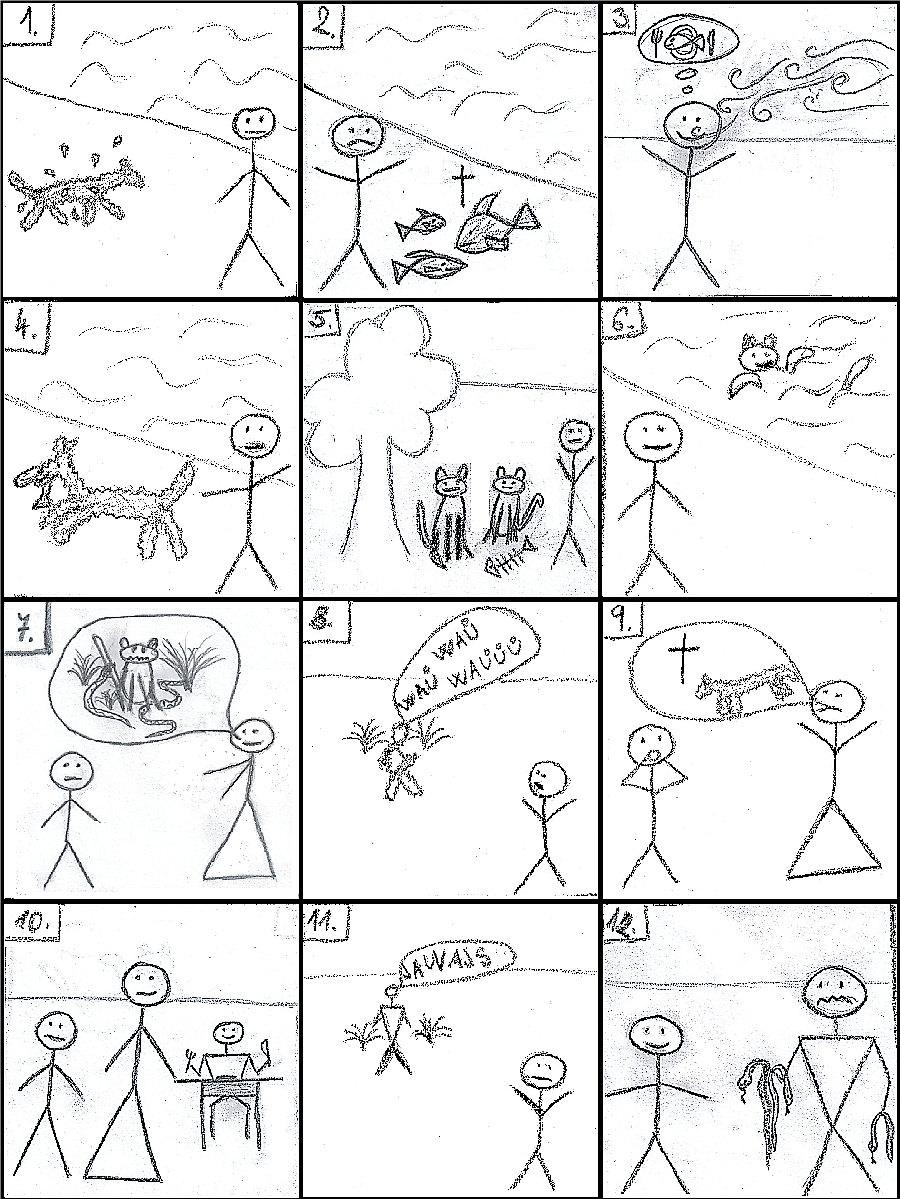
\includegraphics[width=\linewidth]{images/Tariana_main.png}
\vfill

\begin{assgts}
\item \detcorr
\item How would Jovino describe the following situations in Tariana?

\begin{tabular}{@{}r@{~}lr@{~}l@{}}
    \multicolumn{2}{c}{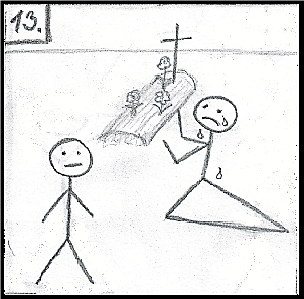
\includegraphics[width = 3.5 cm]{images/Tariana_13.png}} & \multicolumn{2}{c}{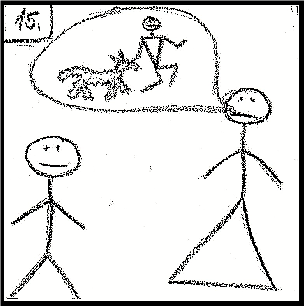
\includegraphics[width = 3.5 cm]{images/Tariana_15.png}} \\
    13. & \texttr{Her cat died.} & 15. & \texttr{Her husband stole their dog.} \\[0.8em]
    \multicolumn{2}{c}{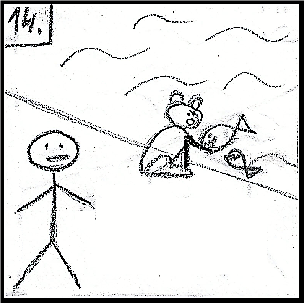
\includegraphics[width = 3.5 cm]{images/Tariana_14.png}} & \multicolumn{2}{c}{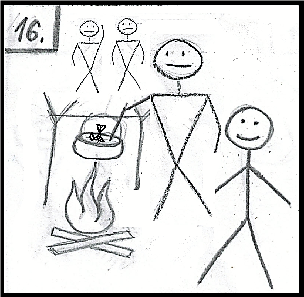
\includegraphics[width = 3.5 cm]{images/Tariana_16.png}} \\
    14. & \texttr{The fish\pl\ bit my cat.} & 16. & \texttr{The men cooked my fish\sg.} \\
\end{tabular}
\item\sloppy Translate into English the following sentences and explain in which situation might Jovino utter them:

\begin{enumerate}[start = 17]
    \item \cmubdata{dihã tʃinune nañhamahka}
    \item \cmubdata{pisana nahã kuphene diinuka}
    \item \cmubdata{mawaɾi tʃãɾi diwhãsika}
    \item \cmubdata{duhã kuphene nañhapidaka}
\end{enumerate}
\end{assgts}
\end{problem}

\begin{problem}{\langnameGee}{\namePHelmer}{\LOYear{\RoLOAbbr}{2018}}
\IntroVerbs{\langnameGee}\ \IntroAndEnglishRandom:

    \begin{longtable}{rl@{\hskip0.5in}cl}
        \chaosline{baipaʔmedo}{I came first.}
        \chaosline{baitenedoleʔ}{Will you\pl\ not come first?}
        \chaosline{biʔʃunerisa}{You\sg\ do not go.}
        \chaosline{biʔteme}{You\pl\ will only talk.}
        \chaosline{biʔtemirisadoleʔ}{I only ran.}
        \chaosline{dospaʔmi}{Will I not go?}
        \chaosline{dospaʔmiduʔaleʔ}{Do you\pl\ only run?}
        \chaosline{dosʃuneduʔa}{You\sg\ only talked.}
        \chaosline{dosʃuneduʔadoleʔ}{You\sg\ will not come.}
        \chaosline{meʔpaʔmerisaleʔ}{Do you\sg\ talk first?}
        \chaosline{meʔʃumeduʔa}{Did I not just run?}
        \chaosline{meʔtemiduʔa}{You\pl\ run.}
    \end{longtable}

\begin{assgts}
\item \detcorr
\item \transinen
\begin{multicols}{2}
\begin{enumerate}[start = 13]
    \item \cmubdata{meʔpaʔmi}
    \item \cmubdata{baiʃune}
    \item \cmubdata{biʔʃunidoleʔ}
    \item \cmubdata{meʔtemeleʔ}
\end{enumerate}
\end{multicols}
\item \transinen[\langnameGee]
\begin{multicols}{2}
\begin{enumerate}[start = 17]
    \item \texttr{Do I talk?}
    \item \texttr{You\sg\ will only run.}
    \item \texttr{You\pl\ did not go first.}
    \item \texttr{Do we just not come?}
    \item \texttr{You\sg\ talk first.}
    \item \texttr{Will I not run first?}
\end{enumerate}
\end{multicols}
\end{assgts}
\end{problem}

\begin{problem}{\langnameGyarung}{\nameSBritova}{\LOYear{\MSKAbbr}{1998}}
\IntroSentences{\langnameGyarung}\ \IntroAndEnglish: 

    \begin{longtable}{rll}
        \sentlineonerow{ŋəñe no tast'on}{We will take care of you\sg.}
        \sentlineonerow{no ŋəñe kəust'oi}{You\sg\ will take care of us.}
        \sentlineonerow{wəjonǯəskə ŋəñe wəst'oi}{They two will take care of us.}
        \sentlineonerow{ŋənǯe ño tast'oñ}{We two will take care of you\pl.}
        \sentlineonerow{wəjoñek nǯo təust'ončh}{They will take care of you two.}
        \sentlineonerow{wəjok ŋəñe wəst'oi}{He will take care of us.}
        \sentlineonerow{wəjok no təust'on}{He will take care of you\sg.}
        \sentlineonerow{wəjonǯəskə ño təust'oñ}{They two will take care of you\pl.}
        \sentlineonerow{ŋəñe ño tast'oñ}{We will take care of you\pl.}
        \sentlineonerow{wəjoñek ŋənǯe wəst'očh}{They will take care of us two.}
        \sentlineonerow{ño ŋa kəust'oŋ}{You\pl\ will take care of me.}
    \end{longtable}

\begin{assgts}
\item \transinen

\begin{enumerate}[start = 12]
\begin{multicols}{2}

    \item \cmubdata{no ŋa kəust'oŋ}
    \item \cmubdata{wəjonǯəskə no təust'on}
    \item \cmubdata{ño ŋənǯe kəust'očh}
\end{multicols}\end{enumerate}
\end{assgts}
\renewcommand \sentlineonerow [2]{\addtocounter{exx}{1}\arabic{exx}.&\cmubdata{#1}&\texttr{#2} \\[0.3em]}

For tasks (b) and (c), you are given the following additional sentences:

\begin{center}
    \begin{tabular}{rl}\setcounter{exx}{14}
        \sentlinetworows{wəjonǯəskə ŋənǯe nɐrə ño t'has wəst'oi}{They two will take care of us two and you\pl\ together.}
        \sentlinetworows{wəjok no nɐrə wəjoñe t'has təust'oñ}{He will take care of you\sg\ and them together.}
        \sentlinetworows{no ŋənǯe nɐrə wəjo t'has kəust'oi}{You\sg\ will take care of us two and him together.}
    \end{tabular}
\end{center}

\begin{assgts}[resume]
\item Here is a Gyarung sentence, in which \textit{a single word} is missing:
\begin{center}
    18. \cmubdata{ŋəñe \_\_\_\_\_\_\_ nɐrə wəjo t'has tast'ončh}
\end{center}
\item[] Fill in the missing word and translate the sentence into English.
\item \transinen[\langnameGyarung]
\begin{enumerate}[start = 19]

    \item \texttr{I will take care of you two.}
    \item \texttr{They two will take care of me.}
    \item \texttr{They will take care of me and you two together.}
    \item \texttr{You\sg\ will take care of me and him together.}
\end{enumerate}
\end{assgts}


\begin{tblsWarning}
\cmubdata{čh}, \cmubdata{ñ}, \cmubdata{ŋ}, \cmubdata{t'}, \cmubdata{t'h} and \cmubdata{ǯ} are consonants; \cmubdata{ɐ} and \cmubdata{ə} are vowels.
\end{tblsWarning}
\end{problem}

\begin{problem}{\langnameHakhun}{\namePArkadiev}{\LOYear{\IOLAbbr}{2018}}
\IntroSentences{\langnameHakhun}\ \IntroAndEnglish:

\begin{center}
    \begin{tabular}{rll}
        \sentlineonerow{ŋa ka kɤ ne}{Do I go?}
        \sentlineonerow{nɤ ʒip tuʔ ne}{Did you\sg\ sleep?}
        \sentlineonerow{ŋabə ati lapkʰi tɤʔ ne}{Did I see him?}
        \sentlineonerow{nirum kəmə nuʔrum cʰam ki ne}{Do we know you\pl?}
        \sentlineonerow{nɤbə ŋa lapkʰi rɤ ne}{Do you\sg\ see me?}
        \sentlineonerow{tarum kəmə nɤ lan tʰu ne}{Did they beat you\sg?}
        \sentlineonerow{nuʔrum kəmə ati lapkʰi kan ne}{Do you\pl\ see him?}
        \sentlineonerow{nɤbə ati cʰam tuʔ ne}{Did you\sg\ know him?}
        \sentlineonerow{tarum kəmə nirum lapkʰi ri ne}{Do they see us?}
        \sentlineonerow{ati kəmə ŋa lapkʰi tʰɤ ne}{Did he see me?}
    \end{tabular}
\end{center}

\begin{assgts}
\item \transinen
\begin{enumerate}[start = 11]
    \item \cmubdata{nɤ ʒip ku ne}
    \item \cmubdata{ati kəmə nirum lapkʰi tʰi ne}
    \item \cmubdata{tarum kəmə nuʔrum cʰam ran ne}
    \item \cmubdata{nirum kəmə tarum lan ki ne}
    \item \cmubdata{nirum kəmə nɤ cʰam tiʔ ne}
    \item \cmubdata{nirum ka tiʔ ne}
\end{enumerate}
\item \transinen[\langnameHakhun]
\begin{multicols}{2}
\begin{enumerate}[start = 17]
    \item \texttr{Did I beat you\sg?}
    \item \texttr{Did they seem me?}
    \item \texttr{Does he know you\sg?}
    \item \texttr{Do you\pl\ sleep?}
\end{enumerate}
\end{multicols}
\end{assgts}

\begin{tblsWarning}
\cmubdata{cʰ}, \cmubdata{kʰ}, \cmubdata{ŋ}, \cmubdata{tʰ}, \cmubdata{ʒ} and \cmubdata{ʔ} are consonants; \cmubdata{ə} and \cmubdata{ɤ} are vowels.
\end{tblsWarning}
\end{problem}

\begin{problem}{\langnameCree}{\nameIDerzhanski}{\LOYear{\MSKAbbr}{2008}}
\IntroVerbs{\langnameCree}\ (in the Plains Cree dialect) \IntroAndEnglish:

\begin{center}
    \begin{tabular}{rll}
        \sentlineonerow{kiwīminahitin}{I want to make you drink.}
        \sentlineonerow{ninanāskomik}{He thanks me.}
        \sentlineonerow{kiwīminahāw}{You want to make him drink.}
        \sentlineonerow{kikīwāpamin}{You saw me.}
        \sentlineonerow{nikīminahikwak}{They made me drink.}
        \sentlineonerow{nikananāskomāw}{I will thank him.}
        \sentlineonerow{kikīnanāskomik}{He thanked you.}
        \sentlineonerow{kikaminahāwak}{You will make them drink.}
    \end{tabular}
\end{center}

\begin{assgts}
\item \transinen
\begin{multicols}{2}
\begin{enumerate}[start = 9]
    \item \cmubdata{niwīwāpamāwak}
    \item \cmubdata{kiminahin}
    \item \cmubdata{ninanāskomikwak}
    \item \cmubdata{kikawāpamik}
\end{enumerate}
\end{multicols}
\item \transinen[\langnameCree]
\begin{multicols}{2}
\begin{enumerate}[start = 13]
    \item \texttr{I saw you.}
    \item \texttr{I want to thank him.}
    \item \texttr{You will thank me.}
    \item \texttr{I make them drink.}
    \item \texttr{He wants to see me.}
    \item \texttr{They see you.}
\end{enumerate}
\end{multicols}
\end{assgts}

\begin{tblsWarning}
A bar above a vowel denotes length.
\end{tblsWarning}
\end{problem}

\begin{problem}{\langnameAinu}{\nameVNeacsu}{\LOYear{\RoLOAbbr}{2021}}
\IntroSentences{\langnameAinu} (in the Shizunai dialect) \IntroAndEnglish:

\begin{center}
    \begin{tabular}{rll}
        \sentlineonerow{ikupa as wa isam}{We drank.}
        \sentlineonerow{inkartek an wa an}{I was glancing.}
        \sentlineonerow{e inkar wa an}{You\sg\ were seeing.}
        \sentlineonerow{inu wa isam}{He listened.}
        \sentlineonerow{iperepa wa oka}{They were feeding.}
        \sentlineonerow{e ipe wa an}{You\sg\ were eating.}
        \sentlineonerow{eci inuruypa wa oka}{You\pl\ were listening a lot.}
        \sentlineonerow{cie koretek wa isam}{We lent you\sg.}
        \sentlineonerow{cieci nukarruypa wa isam}{We stared at you\pl.}
        \sentlineonerow{eun nurepa wa oka}{You\sg\ were telling us.}
        \sentlineonerow{un etekpa wa oka}{He was tasting us.}
        \sentlineonerow{ecien nutek wa an}{You\pl\ were listening to me a little.}
        \sentlineonerow{an yaynu wa isam}{I thought.}
        \sentlineonerow{an eruypa wa oka}{I was devouring them.}
        \sentlineonerow{inuruypa as wa isam}{We listened a lot.}
        \sentlineonerow{en e wa an}{They were eating me.}
        \sentlineonerow{e yaykore wa isam}{You\sg\ gave yourself.}
        \sentlineonerow{cieci nurepa wa oka}{We were telling you\pl.}
    \end{tabular}
\end{center}
\begin{assgts}
\item \transinenall
\begin{multicols}{2}
\begin{enumerate}[start = 19]
    \item \cmubdata{e nukarepa wa isam}
    \item \cmubdata{e koreruy wa an}
    \item \cmubdata{ci yaynukarpa wa oka}
    \item \cmubdata{nuruypa wa isam}
    \item \cmubdata{iperuy an wa isam}
    \blankitem
\end{enumerate}
\end{multicols}
\item \transinen[\langnameAinu]
\begin{enumerate}[label = \arabic*.,start = 24]
    \item \texttr{He was listening to you\pl.}
    \item \texttr{We ate.}
    \item \texttr{You\sg\ were thinking a lot.}
    \item \texttr{They were staring.}
    \item \texttr{We were borrowing him.}
    \item \texttr{I glanced at them.}
    \item \texttr{You\pl\ fed yourselves.}
    \item \texttr{You\sg\ were chattering to us.}
\end{enumerate}
\end{assgts}
\end{problem}

\begin{problem}{\langnameRotokas}{\nameTCucu}{\LOYear{\RoLOAbbr}{2019}}
\IntroVerbs{\langnameRotokas}\ \IntroAndEnglishRandom:
\begin{center}
    \begin{tabular}{rl@{\hskip0.5in}cl}
        \chaosline{aloravirovo}{I went}
        \chaosline{iparaepa}{I threw it}
        \chaosline{ourovo}{I just talked}
        \chaosline{oraoupaveiepa}{I just devoured it}
        \chaosline{orareoveiepo}{I just confessed}
        \chaosline{reoraepo}{he moved it}
        \chaosline{reoraviroepo}{he just took it}
        \chaosline{rupupaveiepo}{we two just discussed}
        \chaosline{rururova}{we two were just swimming}
        \chaosline{vikirava}{we two were getting married}
    \end{tabular}
\end{center}
\begin{assgts}
\item Determine the correct correspondences, knowing that:
\begin{center}
    \begin{tabular}{rcl}
    \cmubdata{oraruruveiepa}&=&\texttr{we two moved ourselves} \\[0.3em]
    \cmubdata{aloparovo}&=&\texttr{he was just eating it} 
    \end{tabular}
\end{center}
\item \transinen
\begin{multicols}{2}
\begin{enumerate}[start = 11]
    \item \cmubdata{rupuraepo}
    \item \cmubdata{ouparava}
    \item \cmubdata{reoparoepa}
    \item \cmubdata{oraruruveviroepa}
\end{enumerate}
\end{multicols}
\item \transinen[\langnameRotokas]
\begin{enumerate}[start = 15]
    \item \texttr{I was devouring him}
    \item \texttr{he was just getting married}
    \item \texttr{we two just jumped}
    \item \texttr{we two arrived}
    \item \texttr{we two ate it}
    \blankitem
\end{enumerate}
\end{assgts}
\end{problem}

\begin{problem}{\langnameDinka}{\nameMLaznicka}{\LOYear{\CLOAbbr}{2019}}
\IntroSentences{\langnameDinka} (in the Agar dialect) \IntroAndEnglish: 

\begin{tabular}{rll}
  \sentlineonerow{dàam báng}{Do I catch the chief?}
  \sentlineonerow{báng àdɔ́ɔm jò}{It's the chief that the dog catches.}
  \sentlineonerow{rów àpíik wèng}{It's the hippo that the cow pushes.}
  \sentlineonerow{rów àdɔ̀m jó}{The hippo catches the dog.}
  \sentlineonerow{tɛ̀ɛɛt wéng}{Do I curse the cow?}
  \sentlineonerow{ghɛ̂ɛn àgèl rów}{I protect the hippo.}
  \sentlineonerow{tèeet kwàc ghɛ̂ɛn}{Does the leopard curse me?}
  \sentlineonerow{gèeet bàng jó}{Does the chief cook the dog?}
  \sentlineonerow{jó àgéeet bàng}{It's the dog that the chief cooks.}
  \sentlineonerow{gèel jò kwác}{Does the dog protect the leopard?}
  \sentlineonerow{jó àlɔ̀ɔk ê}{The dog washes him.}
  \sentlineonerow{gɔ̀ɔɔr kwác}{Do I seek the leopard?}
  \sentlineonerow{báng àgòor kwác}{The chief seeks the leopard.}
  \sentlineonerow{rów àwèc wéng}{The hippo hits the cow.}
  \sentlineonerow{wéng àwèc ê}{The cow hits him.}
\end{tabular}

\begin{assgts}
\item \transinen[\langnameDinka]
\end{assgts}
\begin{enumerate}[noitemsep, start = 16]

    \item \texttr{I cook the leopard.}
    \item \texttr{Do I cook the dog?}
    \item \texttr{The leopard washes the hippo.}
    \item \texttr{It's the leopard that the chief washes.}
    \item \texttr{Do I wash the chief?}
    \item \texttr{I hit him.}
    \item \texttr{Does the hippo push the dog?}
    \item \texttr{Does the cow hit the dog?}
    \item \texttr{The chief curses him.}
    \item \texttr{It's me that the hippo protects.}
\end{enumerate}

\begin{tblsWarning}\largerpage  
Vowel doubling and tripling denotes length (short \cmubdata{a}, medium \cmubdata{aa}, long \cmubdata{aaa}). The marks {\char"25CC\char"300}, {\char"25CC\char"301}, and {\char"25CC\char"302} above the vowel denote low, high, and falling tones respectively.

\cmubdata{ɛ} and \cmubdata{ɔ} are vowels similar to \cmubdata{e} and \cmubdata{o} respectively, but pronounced with a more open mouth (but less open than \cmubdata{a}). 

The language features two types of vowel phonation, but they were not included in the problem for simplicity.
\end{tblsWarning}
\end{problem}

\hypertarget{solutions-of-practice-problems}{%
\section{Solutions of practice problems}}

\begin{practiceproblemsolution}{6.7. \langnameSwahili}

\begin{solutions}[label=Solution 6.7\alph*]
    \item Set I:
    \begin{multicols}{5}
        \begin{enumerate}
            \item A.
            \item B.
            \item K.
            \item L.
            \item D.
            \item C.
            \item E.
            \item F.
            \item J.
            \item M.
            \item N.
            \item G.
            \item H.
            \item I.
            \item[]
        \end{enumerate}
    \end{multicols}
    \item[] Set II:
    \begin{multicols}{5}
        \begin{enumerate}[start = 15, label = \arabic*.]
            \item O.
            \item Z.
            \item Y.
            \item Q.
            \item P.
            \item W.
            \item X.
            \item U.
            \item V.
            \item AA.
            \item R.
            \item S.
            \item T.
        \end{enumerate}
    \end{multicols}
    \item
\begin{enumerate}[label = \arabic*., start = 28]
\begin{multicols}{3}
    \item \cmubdata{unatembelea}
    \item \cmubdata{hutembelei}
    \item \cmubdata{hukutembelea}
    \item \cmubdata{utatembelea}
    \item \cmubdata{anakufa}
    \item \cmubdata{hafi}
    \item \cmubdata{alikufa}
    \item \cmubdata{hatakufa}
    \item[] \vphantom{x}
\end{multicols}\end{enumerate}
\end{solutions}

\rules

\begin{enumerate}
    \item Negation: \cmubdata{ha-}
    \item Subject: 
    \begin{table}[H]
    \begin{tabular}{ lccc }
    \lsptoprule
    & 1 & 2 & 3 \\ \midrule
    \textsc{sg} & \cmubdata{ni} & \cmubdata{u} &\cmubdata{a}\\
    \textsc{pl} & \cmubdata{tu} & \cmubdata{m} & \cmubdata{wa} \\
    \lspbottomrule
    \end{tabular}
    \end{table}
    \item Tense/Negation: 
    \begin{table}[H]
    \begin{tabular}{ lccc }
    \lsptoprule
    & Past & Present & Future \\\midrule
    Affirmative & \cmubdata{li} & \cmubdata{na} & \cmubdata{ta}\\
    Negative & \cmubdata{ku} & $\varnothing$ & \cmubdata{ta}\\
    \lspbottomrule
    \end{tabular}
    \end{table}
    \item Stem
    \item[] Other changes:
    \begin{itemize}

        \item Negative marker can merge with the subject marker:
        \begin{itemize}

            \item \cmubdata{ha- $+$ -ni- \rightarrow\ si-}
            \item \cmubdata{ha- $+$ -V- \rightarrow\ hV-} \quad\quad (\cmubdata{V $=$ a} or \cmubdata{u})
        \end{itemize}
        \item For present negative:
        \begin{itemize}

            \item last vowel of the stem (\cmubdata{a}) becomes \cmubdata{i}.
            \item if the stem starts with the morpheme \cmubdata{ku-}, it gets dropped.
        \end{itemize}
    \end{itemize}
\end{enumerate}

\end{practiceproblemsolution}

\begin{practiceproblemsolution}{6.8. \langnameTariana}

\begin{solutions}[label=Solution 6.8\alph*]
    \item
        \begin{enumerate}[leftmargin = 1em]
        \begin{multicols}{6}

            \item G.
            \item I.
            \item B.
            \item L.
            \item A.
            \item C.
            \item F.
            \item D.
            \item J.
            \item K.
            \item H.
            \item E.
       \end{multicols} \end{enumerate}
    \item \begin{enumerate}[start = 13]

        \item \cmubdata{duhã pisana diyãmisika}
        \item \cmubdata{kuphene nuhã pisana nawhãka}
        \item \cmubdata{duhã tʃãɾi nahã tʃinu diitupidaka}
        \item \cmubdata{tʃãɾine nuhã kuphe nayanaka}
    \end{enumerate}
    \item \begin{enumerate}[start = 17]

        \item \texttr{His dogs ate.} (Jovino heard the dogs eating, tearing the meat.)
        \item \texttr{The cat killed their fish\pl.} (Jovino witnessed the action.)
        \item \texttr{The snake bit the man.} (Jovino saw the bleeding wound.)
        \item \texttr{Her fish\pl\ ate.} (Someone told that to Jovino.)
    \end{enumerate}
\end{solutions}

\rules
\begin{itemize}
    \item Word order: SOV, Possessor-Possessed
    \item Possessives: \cmubdata{nuhã} = 1\textsc{sg}, \cmubdata{dihã} = 3\textsc{sg} masc, \cmubdata{duhã} = 3\textsc{sg} fem, \cmubdata{nahã} = 3\textsc{pl}
    \item \cmubdata{-ne} = plural (for nouns)
    \item Verb:
    \begin{enumerate}

        \item Subject number (\cmubdata{di-} = \textsc{sg}, \cmubdata{na-} = \textsc{pl})
        \item Stem
        \item Evidential markers:
        \begin{itemize}

            \item $\varnothing$ = visual (Jovino was a witness.)
            \item \cmubdata{-mah-} = sensory non-visual (hearing/smell)
            \item \cmubdata{-si-} = inferential (Jovino sees the result of the action.)
            \item\sloppy \cmubdata{-pida-} = reportative (Jovino finds out about it from someone else.)
        \end{itemize}
        \item \cmubdata{-ka} -- Alternatively, this mark can be combined with the evidential markers, resulting in: \cmubdata{-ka}, \cmubdata{-mahka}, \cmubdata{-sika}, \cmubdata{-pidaka}).
    \end{enumerate}
\end{itemize}
\end{practiceproblemsolution}

\begin{practiceproblemsolution}{6.9. \langnameGee}

\begin{solutions}[label=Solution 6.9\alph*]
    \item
        \begin{enumerate}
        \begin{multicols}{5}
            \item C.
            \item F.
            \item A.
            \item I.
            \item B.
            \item L.
            \item G.
            \item E.
            \item K.
            \item J.
            \item H.
            \item D.
       \end{multicols} \end{enumerate}
    \item \begin{enumerate}[start = 13]
        \item \texttr{You\pl\ talk.}
        \item \texttr{Did we not come?}
        \item \texttr{I went.}
        \item \texttr{Will you\sg\ talk?}

    \end{enumerate}
    \item \begin{enumerate}[start = 17]
        \item \cmubdata{meʔpaʔneleʔ}
        \item \cmubdata{dostemeduʔa}
        \item \cmubdata{baiʃumirisado}
        \item \cmubdata{biʔpaʔniduʔadoleʔ}
        \item \cmubdata{meʔpaʔmerisa}
        \item \cmubdata{dostenerisadoleʔ}
    \end{enumerate}
\end{solutions}

\rules

\begin{table}[H]
    \begin{tabular}{lllllll}
    \lsptoprule
          &           & \multicolumn{2}{c}{Subject} &   &   &  \\\cmidrule(lr){3-4}
    {Stem} & {Tense} & Pers. & Number & {Adverb} & {Neg} & {Q} \\\midrule
    \begin{tabular}{@{}c@{}}
         \cmubdata{biʔ} (\texttr{come}) \\ \cmubdata{bai} (\texttr{go}) \\ \cmubdata{dos} (\cmubdata{run}) \\ \cmubdata{meʔ} (\texttr{talk}) \\
    \end{tabular}&
    \begin{tabular}{@{}c@{}}
         \cmubdata{ʃu} (past) \\ \cmubdata{paʔ} (present) \\ \cmubdata{te} (future) \\
    \end{tabular}&
    \begin{tabular}{@{}c@{}}
         \cmubdata{n} (1) \\ \cmubdata{m} (2) \\
    \end{tabular}&
    \begin{tabular}{@{}c@{}}
         \cmubdata{e} (\textsc{sg}) \\ \cmubdata{i} (\textsc{pl}) \\
    \end{tabular}&
    \begin{tabular}{@{}c@{}}
         \cmubdata{duʔa} (\texttr{only}) \\ \cmubdata{risa} (\texttr{first}) \\
    \end{tabular}&
    \begin{tabular}{@{}c@{}}
         \cmubdata{do} \\
    \end{tabular}&
    \begin{tabular}{@{}c@{}}
         \cmubdata{leʔ} \\
    \end{tabular}\\
    \lspbottomrule
    \end{tabular}
\end{table}
\end{practiceproblemsolution}

\begin{practiceproblemsolution}{6.10. \langnameGyarung}

\begin{solutions}[label=Solution 6.10\alph*]
    \item \begin{enumerate}[start = 12]

        \item \texttr{You\sg\ will take care of me.}
        \item \texttr{They two will take care of you\sg.}
        \item \texttr{You\pl\ will take care of us two.}
    \end{enumerate}
    \item 18. Missing word: \cmubdata{no} \\ \hphantom{18.} Translation: \texttr{We will take care of you\sg\ and him together.}
    \item \begin{enumerate}[start = 19]

        \item \cmubdata{ŋa nǯo tast'ončh}
        \item \cmubdata{wəjonǯəskə ŋa wəst'oŋ}
        \item \cmubdata{wəjoñek ŋa nɐrə nǯo t'has wəst'oi}
        \item \cmubdata{no ŋa nɐrə wəjo t'has kəust'očh}
    \end{enumerate}
\end{solutions}

\rules
\begin{itemize}
    \item Structure: \fbox{S O (\cmubdata{nɐrə} O' \cmubdata{t'has}) V} \\ For complex sentences, V refers to the sum of the objects (you\sg\ + me = us two; you\sg\ + us two = us; him + you\sg\ = you two, etc.)
    \item Pronouns (S = O):
    \begin{table}[H]
    \begin{tabular}{ cccc }
    \lsptoprule
         & \textsc{sg} & \textsc{du} & \textsc{pl} \\\midrule
         1 & \cmubdata{ŋa} & \cmubdata{ŋənǯe} & \cmubdata{ŋañe} \\
         2 & \cmubdata{no} & \cmubdata{nǯo} & \cmubdata{ño} \\
         3 & \cmubdata{wəjok}\textsuperscript{\dag} & \cmubdata{wəjonǯəskə} & \cmubdata{wəjoñek}\textsuperscript{\dag} \\
         \lspbottomrule
    \end{tabular}
         \footnotetext{\textsuperscript{\dag} final \cmubdata{k} is dropped if it's an object}
    \end{table}
    \item Verb:
    \begin{enumerate}

        \item Information about 2nd person: \cmubdata{t} = O2, \cmubdata{k} = S2, \cmubdata{w} = $\nexists$2
        \item Subject and object person: \cmubdata{a} = S1--O2, \cmubdata{ə} = S3--O1, \cmubdata{ə} = S2--O1 or S3--O2

     \end{enumerate}
\end{itemize}
        \note{An alternative (and simpler) explanation can combine the first two morphemes into one. We can write: \cmubdata{ta} = S1--O2, \cmubdata{təu} = S3--O2, \cmubdata{wə} = S3--O1, \cmubdata{kəu} = S2--O1.}

\begin{itemize}
    \item []\hphantom{abc}
    \begin{enumerate}[start = 3]

        \item \cmubdata{st'o} -- it most likely represents the stem, possibly including the TAM marker
        \item Information about the subject: 
        \begin{table}[H]
        \begin{tabular}{ cccc }
         \lsptoprule
         & \textsc{sg} & \textsc{du} & \textsc{pl} \\ \midrule
         1 & \cmubdata{ŋ} & \cmubdata{čh} & \cmubdata{i} \\
         2 & \cmubdata{n} & \cmubdata{nčh} & \cmubdata{ñ} \\
         \lspbottomrule
    \end{tabular}
    \end{table}
     \end{enumerate}
\end{itemize}
\end{practiceproblemsolution}

\begin{practiceproblemsolution}{6.11. \langnameHakhun}

\begin{solutions}[label=Solution 6.11\alph*]
    \item
\begin{enumerate}[start = 11]
    \item \texttr{Do you\sg\ sleep?}
    \item \texttr{Did he see us?}
    \item \texttr{Do they know you\pl?}
    \item \texttr{Do we beat them?}
    \item \texttr{Did we know you\sg?}
    \item \texttr{Did we go?}
\end{enumerate}
\item
\begin{enumerate}[start = 17]
    \item \cmubdata{ŋabə nɤ lan tɤʔ ne}
    \item \cmubdata{tarum kəmə ŋa lapkʰi tʰɤ ne}
    \item \cmubdata{ati kəmə nɤ cʰam ru ne}
    \item \cmubdata{nuʔrum ʒip kan ne}
\end{enumerate}
\end{solutions}

\rules
\begin{itemize}
    \item Word order: S O V X \cmubdata{ne}
    \item S: in transitive sentences, it receives the suffix \cmubdata{-bə} (if S is 1\textsc{sg} or 2\textsc{sg}) or the word \cmubdata{kəmə} placed after the subject (otherwise).
    \item X: hierarchy 1 > 2 > 3:\\
    \begin{tabular}[t]{ll @{\quad\quad} ll}
    \lsptoprule
    \cmubdata{t-   -ʔ} & past, S>O  & \cmubdata{ɤ} & $\exists$1\textsc{sg} \\
    \cmubdata{tʰ-} & past, S<O  & \cmubdata{i} & $\exists$1\textsc{pl}\\
    \cmubdata{k-} & present, S>O & \cmubdata{u} & $\nexists$1 \& $\exists$2\textsc{sg}\\
    \cmubdata{r-} & present, S>O  & \cmubdata{an} & $\nexists$1 \& $\exists$2\textsc{pl} \\
    \lspbottomrule
    \end{tabular}
\end{itemize}

\end{practiceproblemsolution}

\begin{practiceproblemsolution}{6.12. \langnameCree}

\begin{solutions}[label=Solution 6.12\alph*]
    \item
\begin{enumerate}[start = 9]
\begin{multicols}{2}
    \item \texttr{I want to see them.}
    \item \texttr{You make me drink.}
    \item \texttr{They thank me.}
    \item \texttr{He will see you.}
\end{multicols}\end{enumerate}
\item
\begin{enumerate}[start = 13]
\begin{multicols}{2}
    \item \cmubdata{kikīwāpamitin}
    \item \cmubdata{niwīnanāskomāw}
    \item \cmubdata{kikananāskomin}
    \item \cmubdata{niminahāwak}
    \item \cmubdata{niwīwāpamik}
    \item \cmubdata{kiwāpamikwak}
\end{multicols}\end{enumerate}
\end{solutions}

\rules

\paragraph*{Option 1 -- Detailed}

\begin{enumerate}
    \item Existence of 2\textsc{sg}:

        \begin{itemize}

        \begin{multicols}{2}
            \item \cmubdata{ki} = exists (S or O)
            \item \cmubdata{ni} = does not exist
        \end{multicols}	\end{itemize}
    \item TAM markers:

 \begin{multicols}{2}
        \begin{itemize}

            \item \cmubdata{wī} = volitive (\texttr{to want to})
            \item \cmubdata{kī} = past
            \item $\varnothing$ = present
            \item \cmubdata{ka} = future
        \end{itemize}
    \end{multicols}
    \item Stem

 \begin{multicols}{2}
        \begin{itemize}

            \item \wordtrans{minah}{to make drink}
            \item \wordtrans{nanāskom}{to thank}
            \item \wordtrans{wāpam}{to see}
        \end{itemize}
    \end{multicols}
    \item Information about 3\textsuperscript{rd} person

\begin{multicols}{2}
        \begin{itemize}

            \item \cmubdata{ik} = S3\textsc{sg}
            \item \cmubdata{ikwak} = S3\textsc{pl}
            \item \cmubdata{āw} = O3\textsc{sg}
            \item \cmubdata{āwak} = O3\textsc{pl}
            \item \cmubdata{in} = $\nexists$3 \& S2\textsc{sg}
            \item \cmubdata{itin} = $\nexists$3 \& O2\textsc{sg}
        \end{itemize}
    \end{multicols}
\end{enumerate}

\paragraph*{Option 2 -- Condensed}\quad\\
\begin{table}[H]
    \begin{tabular}{cccc}
    \lsptoprule
    2\textsuperscript{nd} pers. & TAM & Stem & S/O \\
    \midrule
    \begin{tabular}{@{}l@{}}
        $\exists$ \rightarrow\ \cmubdata{ki} \\
        $\nexists$ \rightarrow\ \cmubdata{ni}
    \end{tabular} &
    \begin{tabular}{@{}l@{}}
        $\varnothing$ = present \\ \cmubdata{wī} = volitive \\ \cmubdata{kī} = past \\ \cmubdata{ka} = future\\
    \end{tabular} &
    \begin{tabular}{@{}l@{}}
         \wordtrans{minah}{to make drink} \\ \wordtrans{nanāskom}{to thank}
            \\\wordtrans{wāpam}{to see}\\
    \end{tabular} &
    \begin{tabular}{@{}l@{}}
         \cmubdata{-ik}(\cmubdata{wak}) = S3\textsc{sg}(\textsc{pl}) \\
         \cmubdata{-āw}(\cmubdata{ak}) = O3\textsc{sg}(\textsc{pl}) \\
         \cmubdata{-in} = $\nexists$3 \& S2\textsc{sg}\\
        \cmubdata{-itin} = $\nexists$3 \& O2\textsc{sg}	\\
    \end{tabular}\\\lspbottomrule
    \end{tabular}
\end{table}
\end{practiceproblemsolution}

\begin{practiceproblemsolution}{6.13. \langnameAinu}

\begin{solutions}[label=Solution 6.13\alph*]
    \item \begin{enumerate}[start = 19]

        \item \texttr{You\sg\ showed them.}
        \item \texttr{He was giving a lot to you\sg.} / \texttr{They were giving a lot to you\sg.} / \texttr{You\sg\ were giving a lot to him.} \\ You can also use other ways to express \texttr{give a lot}, such as \texttr{be generous} etc.
        \item \texttr{We were seeing ourselves.}
        \item \texttr{He listened a lot to them.} / \texttr{They listened a lot to them.}
        \item \texttr{I ate a lot.}
    \end{enumerate}
    \item \begin{enumerate}[start = 24, label = \arabic*.]
    \item \cmubdata{eci nupa wa oka}
    \item \cmubdata{ipepa as wa isam}
    \item \cmubdata{e yaynuruy wa an}
    \item \cmubdata{inkarruypa wa oka}
    \item \cmubdata{ci koretekre wa an}
    \item \cmubdata{an nukartekpa wa isam}
    \item \cmubdata{eci yayerepa wa isam}
    \item \cmubdata{eun nureruypa wa oka}
    \end{enumerate}
    \end{solutions}
\rules
\begin{itemize}
    \item \emph{Tense/Aspect}: placed at the end of the structure.

        \begin{itemize}

        \item past simple (perfective): \cmubdata{wa isam}
        \item past continuous (imperfective):

        \begin{itemize}

        \item \cmubdata{wa an} – if the verb is considered singular\footnote{The plurality of the verb is determined by the subject (for intransitive verbs) or by the object (for transitive verbs). In other words, the verb plurality follows an ergative marking -- see \sectref{morphoalign}.}
        \item \cmubdata{wa oka} – if the verb is considered plural\footnote{See previous footnote.}
        \end{itemize}
        \end{itemize}
        \item \emph{Pronoun markers} 
        \begin{table}[H]
            \begin{tabular}{cccc}
                \lsptoprule
                Person & S (Intransitive) & S (Transitive) & Object \\ \midrule
                1 sg & \cmubdata{-an} & \cmubdata{an-} & \cmubdata{en-} \\ 
                2 sg & \cmubdata{e-} & \cmubdata{e-} & \cmubdata{e-} \\ 
                3 sg & $\varnothing$ & $\varnothing$ & $\varnothing$ \\ 
                1 pl & \cmubdata{-as} & \cmubdata{ci-} & \cmubdata{un-} \\ 
                2 pl & \cmubdata{eci-} & \cmubdata{eci-} & \cmubdata{eci-} \\ 
                3 pl & $\varnothing$ & $\varnothing$ & $\varnothing$ \\ 
                \lspbottomrule
            \end{tabular}
        \end{table}
\item[] The hyphen that precedes or follows the morpheme shows its position with respect to the verb (before or after). In the case of transitive verbs, if both arguments are placed before the verb, they are placed in the order subject – object and they fuse together into a single word.
\item \emph{Marker for verb plurality} (as defined above): suffix \cmubdata{-pa} is placed after the verbal affixes (if any).
\item \emph{Verbal affixes}:

        \begin{itemize}

        \item \cmubdata{yay-} = reflexive (\texttr{to think} = \texttr{to hear yourself})
        \item \cmubdata{-ruy} = intensifier (can be translated by \texttr{a lot}, but it can also be lexicalised in the choice of verb: \texttr{to eat} – \texttr{to devour}, \texttr{to see} – \texttr{to stare})
        \item \cmubdata{-tek} = mitigator (the opposite of \cmubdata{-ruy}: \texttr{to eat} – \texttr{to taste}, \texttr{to see} – \texttr{to glance})
        \item \cmubdata{–(r)e}: causative (\texttr{to eat} \rightarrow\ to make someone eat = \texttr{to feed}, \texttr{to see} \rightarrow\ to make someone see = \texttr{to show}). Additionally, \cmubdata{-re \rightarrow\ e / r \_}
        \end{itemize}
    \item \emph{Verbal stems}: Each verb has two different stems, for transitive and intransitive:\largerpage[2]
        \begin{table}[H]
            \begin{tabular}{lll}
            \lsptoprule
                English & Intransitive & Transitive \\ \midrule
                \texttr{to eat} & \cmubdata{ipe} & \cmubdata{e} \\ 
                \texttr{to see} & \cmubdata{inkar} & \cmubdata{nukar} \\ 
                \texttr{to listen} & \cmubdata{inu} & \cmubdata{nu} \\ 
                \texttr{to drink} & \cmubdata{iku} &  \\ 
                \texttr{to give} &  & \cmubdata{kore}\footnote{In reality, the stem \cmubdata{kore} (\texttr{to give}) comes from the stem \cmubdata{kor} (\texttr{to have}) + causative marker (\texttr{to have} \rightarrow\ to make someone have = \texttr{to give}).}\\
            \lspbottomrule
            \end{tabular}
        \end{table}
\end{itemize}

\end{practiceproblemsolution}
\begin{practiceproblemsolution}{6.14. \langnameRotokas}

\begin{solutions}[label=Solution 6.14\alph*]
    \item
        \begin{enumerate}[leftmargin = 1em]
        \begin{multicols}{5}

            \item D.
            \item A.
            \item G.
            \item J.
            \item H.
            \item C.
            \item E.
            \item I.
            \item F.
            \item B.
       \end{multicols} \end{enumerate}
    \item \begin{enumerate}[start = 11]
        
        \item \texttr{I just swam}
        \item \texttr{I was taking him}
        \item \texttr{he was talking}
        \item \texttr{we two emigrated}

    \end{enumerate}
    \item \begin{enumerate}[start = 15]

        \item \cmubdata{aloparavirova}
        \item \cmubdata{oraouparoepo}
        \item \cmubdata{oravikiveiepo}
        \item \cmubdata{ipaveviroepa}
        \item \cmubdata{aloveva}
    \end{enumerate}
\end{solutions}

\rules
\begin{enumerate}
    \item \cmubdata{ora-} = reciprocal / reflexive (\texttr{to move} \rightarrow\ \texttr{to move oneself}; \texttr{to take} \rightarrow\ to take oneself = \texttr{to marry}; \texttr{to speak} \rightarrow\ \texttr{to discuss}; \texttr{to throw} \rightarrow\ \texttr{to jump});
    \item Stem: \wordtrans{-alo-}{to eat}, \wordtrans{-ipa-}{to go}, \wordtrans{-ou-}{to take}, \wordtrans{-reo-}{to speak}, \wordtrans{-rupu-}{to swim}, \wordtrans{-ruru-}{to move}, \wordtrans{-viki-}{to throw};
    \item \cmubdata{-pa-} = imperfect (progressive aspect);
    \item Subject: \cmubdata{-ra-} = 1\textsc{sg}, \cmubdata{-ro-} = 3\textsc{sg}, \cmubdata{-ve-} = 1d;
    \item \cmubdata{-viro-} = intensifier / to do till the end (\texttr{to eat} \rightarrow\ \texttr{to devour}; \texttr{to talk} \rightarrow\ \texttr{to confess}; \texttr{to walk} \rightarrow\ \texttr{to arrive} = to walk till the end; \texttr{to move oneself} \rightarrow\ \texttr{to emigrate});
    \item Transitivity: \cmubdata{-v-} = transitive, \cmubdata{-(i)ep-} = intransitive (\cmubdata{ep \rightarrow\ iep / e \_)};
    \item \cmubdata{-a} = far past, \cmubdata{-o} = recent past (\texttr{just}).
\end{enumerate}
\note{In this language, the reflexive is considered intransitive (it takes the marker \cmubdata{-ep-}), while in Ainu (previous problem), the reflexive is considered transitive (it uses the transitive form of the stem).}
\end{practiceproblemsolution}


\begin{practiceproblemsolution}{6.15. \langnameDinka}

\begin{solutions}[label=Solution 6.15\alph*]
    \item \begin{enumerate}[start = 16]
%             \begin{multicols}{2}
                \item \cmubdata{ghɛ̂ɛn àgèet kwác}
                \item \cmubdata{gɛ̀ɛɛt jó}
                \item \cmubdata{kwác àlɔ̀ɔk rów}
                \item \cmubdata{kwác àlɔ́ɔɔk bàng}
                \item \cmubdata{làaak báng}
                \item \cmubdata{ghɛ̂ɛn àwèc ê}
                \item \cmubdata{pìik ròw jó}
                \item \cmubdata{wèec wèng jó}
                \item \cmubdata{báng àtèet ê}
                \item \cmubdata{ghɛ̂ɛn àgéel ròw}
%             \end{multicols}
        \end{enumerate}
\end{solutions}

\rules
\begin{itemize}
    \item Sentence structure:

    \begin{itemize}

        \item Active (e.g., \texttr{The dog catches the hippo.}) – word order \fbox{S V O}
        \item Active with focused object (e.g., \texttr{It's the hippo that the dog catches.}) – word order \fbox{O V S}; \\ the tone of the subject becomes low.
        \item Interrogative (e.g., \texttr{Does the dog catch the hippo?}) – word order \fbox{V S O}; \\the tone of the subject becomes low.
\end{itemize}
	\pagebreak
	\item Verb

 \begin{description}

     \item[Stems:] ~

     \begin{multicols}{4}
         \item[] \wordtrans{dɔ̀m}{to catch}
         \item[] \wordtrans{gèl}{to protect}
         \item[] \wordtrans{gèet}{to cook}
         \item[] \wordtrans{gòor}{to seek}
         \item[] \wordtrans{lɔ̀ɔk}{to wash}
         \item[] \wordtrans{pìk}{to push}
         \item[] \wordtrans{tèet}{to curse}
         \item[] \wordtrans{wèc}{to hit}
     \end{multicols}
     \item[Active:] ~\\
     Add prefix \cmubdata{à-}.
     \item[Interrogative:]~\\
     Vowels lengthen by one degree (short \rightarrow\ medium \rightarrow\ long). \\
      If the subject is 1\textsc{sg}, vowel opens by one degree (\cmubdata{i} \rightarrow\ \cmubdata{e} \rightarrow\ \cmubdata{ɛ} \rightarrow\ \cmubdata{a} and \cmubdata{u} \rightarrow\ \cmubdata{o} \rightarrow\ \cmubdata{ɔ} \rightarrow\ \cmubdata{a}).
     \item[Active (focused object):]~\\
     Add prefix \cmubdata{à-}.\\
     The vowel lengthens by one degree. \\
     The tone becomes high.
\end{description}
\end{itemize}
\end{practiceproblemsolution}

% \section{Further reading}
% \begin{enumerate}[{label=[\arabic{*}]}]
%     \item Donohue, Mark and Wichmann, Søren (ed,). “The typology of semantic alignment.”\ \textit{Oxford University Press}, Oxford (2005).
%     \item  Fortescue, Michael and Mithun, Marianne and Evans, Nicholas (ed.). “The Oxford handbook of polysynthesis.”\ \textit{Oxford University Press}, Oxford (2017).
%     \item  Hengeveld, Kees and Narrog, Heiko and Olbertz, Hella. “The grammaticalization of tense, aspect, modality and evidentiality.”\ \textit{De Gruyter Mouton}, Berlin (2017).
% \end{enumerate}
\nocite{DonohueWichmann2005, FortescueEtAl2017, HengeveldEtAl2017}
% \printbibliography[heading=FurtherReading]
\FurtherReadingBox{}
\end{refsection}
